\documentclass{article}
\usepackage[includeheadfoot,margin=1.0in]{geometry}
\usepackage{amsfonts}
\usepackage{amsmath}
\usepackage{amssymb}
\usepackage{fancyhdr}
\usepackage{hyperref}
\usepackage{graphicx}
\usepackage{multicol}
%
% Set Title/Author
%
\title{Software Design Document (SDD)}
\author{Team USA \\ Software Engineering \\ Sam Houston State University}
%
% Set page styles
%
\pagestyle{fancy}
\fancyhead[LE,RO]{SDD}
\fancyhead[RE,LO]{\leftmark}
\fancyfoot[RE,LO]{}
\renewcommand{\headrulewidth}{2pt}
\renewcommand{\thefootnote}{[\arabic{footnote}]}
\begin{document}
%
% Generate Title
%
\maketitle
\newpage
%
% Generate Table of Contents
%
\tableofcontents
\newpage
%
% Begin Design Document Content
%
% Begin preamble with system description
%
\section{Software System Description \& General Introduction}
The software system subject to design and analysis, and referenced throughout this document as ``the system'', or variations thereof, is a two dimensional, point-and-click adventure game. The user takes on the role of a computer science major at Sam Houston State University as they attempt to submit their final lab for Dr. David Burris's Data Structures \& Algorithms course, before the looming deadline. The user will attempt to navigate through various obstacles to complete this objective, while avoiding various traps, hostile entities, and the darkness itself. The game environment consists of 3 levels, occurring on the various floors of Academic Building 1, and in certain other areas on the SHSU campus. Each level consists of individual scenes, containing various entities, collectible items, and textures. The player will navigate through these scenes as they progress through the game. 

The system has been developed using the design techniques in the following sections, and each technique has been evaluated based on the applicable metrics. \textbf{The chosen design methodology for the implementation of the system is object oriented design, using the unified modeling language, or UML.}\footnote{A discussion of why this choice was made occurs in section 8.} Appendix A contains all of the applicable design diagrams, while Appendix B contains all of the applicable storyboard and level progression diagrams. A full sized level progression diagram can be found attached as a supplement to the scaled diagram inside this SDD. 
%
% Design Specifics
%
\section{Design Features \& Specifics} 

	\subsection{Three-Tier}
		The software system itself utilizes a three-tier design, in which there is a separate presentation element for the user to interact with, a separate data processing element, and a data parsing element that will be implemented for persistence between user sessions. 

		\subsubsection{Presentation Element}
			The presentation element for the system consists of the video and audio managers. These receive and handle audio and video requests from the engine module. The application window itself is a standard window as defined by the host computer's operating system, but is abstracted through the use of the SDL2 library. Access to the audio card is also an abstraction provided by SDL2.

		\subsubsection{Data Processing Element}
			The data processing element for the system consists of the engine module and its subordinate transform modules. The engine receives data from the level file and user input. The level file specifies which resources need to be loaded and their associated resource identifiers. The engine can then execute the main loop of the system, which tracks player position versus actor position, items the player has collected, and the player's progression through the game itself. It directs the video and audio manager modules to display the correct and relevant audio and video content to the player via the application window, which comprises the presentation element. 

		\subsubsection{Data Parsing Elements}
			  The system makes use of a two simple file types: save and level files.

        Save files consist of the player's inventory, a level ID, and a scene ID. The engine ensures the player will be able to resume this progress from the last checkpoint that was reached by making requests to the GameSaveSerializer module for loading or saving data as necessary. The save function will occur in a separate thread to ensure gameplay is not interrupted while the player progress is automatically recorded.

        Level files contain a listing of the necessary resources/assets that will be utilized throughout a set of scenes. The Level module will parse a level file and load the resources specified inside of it during its initialization phase; actors and scenes will be stored inside of the Level module itself, while audio and video resources will be loaded and stored by their respective modules.

	\subsection{Multithreading, Deadlocks, and Race Conditions}
    The system implements multithreading in two modules: game saving and audio streaming. Since the system must poll each subsystem during every frame, there are very few instances where multithreading is necessary. Unnecessary multiprocessing was explicitly avoided in the design to reduce complexity and avoid possible deadlock scenarios. It is common practice in the gaming industry to have only one main thread perform most of the work in the program.

    It should be noted that fully multithreaded models were considered during the design process (where video, audio, input, and game logic were each in their own thread). It was decided that the extra performance gained from multithreading did not outweigh the benefits of a less complex design. The chosen design allows for simpler maintenance and modification in the future, while avoiding unnecessarily complex relationships between modules.

    \subsubsection{Streaming Audio}
      The AudioEngine module allows the user to load a single WAV file to stream audio from disk. This audio will play in a loop continually until the next call to stream a file is made. If audio is already streaming and another call to stream audio is made, then the old thread will be stopped and the new stream will take its place. Race conditions cannot occur because only one audio stream can exist at a time and the system cannot communicate with the audio thread once spawned (other than instructing it to halt). Deadlock cannot occur because the audio stream is never polled for data.

    \subsubsection{Game Saving}
      The GameSaveSerializer module allows the user to save and load game progress. The load function is called in a non-threaded context, ensuring that the program cannot progress until the data is retrieved. When the save function is called, a new thread will be spawned and will write the player's progress to disk. This will allow the player's progress to be saved in the background while the rest of the gameplay continues without interruption. The save function will access the save file with options to lock the file for read and write, preventing multiple writes from occuring at the same time. Further, a mutex will be utilized to ensure that the save and load functions are not called while a save function is currently in progress, preventing possible race conditions. Deadlock cannot occur because no thread is polling another thread for data.

  \subsection{Data Organization}
      The system does not save large amounts of data. Therefore, integrating a database would have been a poor design decision that would create unnecessary complexity. Instead, a small save file format will be utilized for persisting player data.

      The save file will store three save slots that will allow the user to store their progress and later resume gameplay. The data will be stored in a binary format to prevent the average player from tampering with it. The data for a single save will be structured as follows:

      \begin{verbatim}
<int level><int scene><int number of inventory items><iteration of int inventory items...>
      \end{verbatim}

	\subsection{Optimization}
      Due to the time constraint of rendering at a consistently high frame rate, most games consider optimization of space to be secondary to optimization of time. However, the game must also store very large resources, like video and audio. This time/space trade-off is a balancing act that should require great care to not over-optimize in either direction, as a wild swing in either direction can make the gameplay a bad experience; too much optimization for time will increase the number of loading zones, which interrupt gameplay, while too much optimization for space will lower the framerate and cause the gameplay to stutter. Therefore, if the system is sufficiently performant after its design, it is best to leave it alone.

		\subsubsection{Optimizing for Time}
      The system will exhibit high cohesion and low coupling after the implementation phase due to object oriented design. This will ensure that each module can be separately optimized without affecting other modules. Inline functions may be utilized for getter and setter methods (which are called frequently) to ensure that unnecessary stack frames are not created in the main loop.

      The linkage of subprograms can be performed in the following order to ensure best performance: GameEngine, Player, BaseActor (followed by the various actors), AudioEngine, VideoEngine, libSDL2. The game loop always begins with a call to SDL2 for mouse input in GameEngine and ends with a call to SDL2 for audio and video in their respective engines; this means we can ensure that the program loads SDL2 in memory at the end of the loop and will be able to utilize SDL2 again at the start of the next looping cycle.

		\subsubsection{Optimizing for Space}
      High cohesion and low coupling will allow the system to be optimized for memory usage in the future if necessary. As mentioned in Optimization for Time, the linkage between modules can be set in a particular order to reduce the number of page faults significantly.

      Images that are to be displayed on screen will be transformed into textures in main memory and then stored in graphics memory during the system's loading phase. This ensures that main memory can free the images immediately after transforming them, allowing the space to be used for other tasks. To further decrease the usage of main memory, the project design forces resources that are not being utilized in a specific level to be released from memory unless explicitly marked as a core component for all levels.

	\subsection{Module Reuse}
		In order to save on development time for future projects, ideally a system should have reusable modules. Regarding this system, the audio and video modules are reusable. They are black boxes that accept .WAV and .PNG files and perform a specific action on those inputs. For the video module, it accepts .PNG files and displays them, while the audio module accepts .WAV files and plays them as sound from attached speakers. This black box design also allows the underlying video and audio functionality provided by SDL2 to be replaced with a different audio/video library without affecting other parts of the system.

    The levels, art assets, and story of the system will all be defined by the level files. This allows the engine to be reused for other point-and-click games with no modification to the existing codebase; the only modified resource will be ASCII text-files.

	\subsection{Implementation Plan}
    The implementation for this project will be written in the C++ programming language, specifically the 2011 standard. The video, audio, and mouse input library utilized to provide basic access to system functions will be SDL2, which is an industry-standard library written and maintained by Valve Corporation. It has been proven and tested thoroughly and is actively used in game development at the time of writing this document. The library will likely be supported and maintained over the course of the next decade by the various companies that utilize it in their applications.
    \subsubsection{Work Distribution}
      All task names are assumed to be modules. Non-module tasks that are distributed will be italicized. Note that some tasks are significantly more complex than others, so these have been distributed out to the developers with more experience in C++. It is expected that each team member will provide assistance to other teammates as necessary if all assigned tasks have been completed. \emph{Note: the following list is two columns for the sake of readability.}
      \begin{multicols}{2}
      \begin{itemize}
        \item Bhandari, Parameshor
        	\begin{itemize}
				\item Main
				\item ResponsiveAudioActor
				\item DelayedAudioActor
				\item AudioStreamActor
				\item VideoActor
				\item \emph{Level files}
			\end{itemize}
        \item Carmona, Juan 
        	\begin{itemize}
				\item MovingActor
				\item ResponsiveVideoActor
				\item VideoEventActor
				\item DelayedVideoActor 
				\item TextboxSpawnActor 
				\item \emph{Level files}
			\end{itemize}
        \item McGowen, Andrew 
        	\begin{itemize}
				\item Level 
				\item \emph{Cross-platform migration} 
				\item \emph{Level files}
			\end{itemize}
        \item Menteer, Derek 
        	\begin{itemize}
				\item AudioEngine
				\item AudioPlayer
				\item VideoEngine
				\item VideoContext 
				\item VideoDisplay
				\item \emph{Level files}
			\end{itemize}
        \item Sanchez, Vincent 
        	\begin{itemize}
				\item GameSaveSerializer 
				\item \emph{Photography \& background texture preparation} 
				\item \emph{Level files}
			\end{itemize}
        \item Sparks, Jordan 
        	\begin{itemize}
				\item Engine
				\item \emph{C++ best practices and guidance} 
				\item \emph{Project quality assurance}
			\end{itemize}
        \item Zhang, John 
        	\begin{itemize}
				\item Player
				\item BaseActor
				\item InventoryItemActor
				\item SceneLink
				\item LevelLink
				\item \emph{Level files}
				\item \emph{Audio tracks \& samples}
			\end{itemize}
      \end{itemize}
      \end{multicols}
      
	\subsection{Final Product Testing}
    Each group of similar modules should have a set of test cases that can be performed to verify their integrity. Testing the modules in isolation will allow developers to ensure their code is correct before attempting to integrate it with other modules. Further, the set of test cases can be utilized to ensure that no new errors have been introduced during maintenance and modification. When compiling code, usage of the \textit{pedantic, force strict standards, and warn on all} flags should be provided to the compiler to ensure that non-standard compliant code is treated as an error; without these flags, the code will not be guaranteed to be cross-platform.

    Team members are encouraged to use the Catch Framework \footnote{See https://github.com/philsquared/Catch for more documentation on the Catch Framework} to write and test for errors in their C++ code, but it is not required. Some modules, such as audio and video, that cannot be completely tested without human interaction will need a custom test file supplied.

    The product should perform smoothly with no errors during the final testing. All possible scenarios in the game should be thoroughly examined multiple times. Use of memory inspection tools, like Valgrind \footnote{See http://valgrind.org/ for more documentation on Valgrind}, should be utilized to ensure that memory leaks do not occur during runtime of the system. Any memory leaks will be considered an error/failure and will need to be resolved before the program is considered acceptable for distribution.
	\subsection{Acceptance Criteria}
		The acceptance criteria for the system defined metrics which must be met for the system to be acceptable for general use. They are:
		\begin{itemize}
			\item Game textures that consume less than 512MB of video memory.
      \item A consistent 60 frames per second on reasonably new graphics cards.
			\item Persistence, implemented through the file system. 
			\item A fully usable application interface, in the form of a window that accepts mouse input consisting of cursor movements and button actuations.
		\end{itemize}
%
% Begin analysis metric definitions
%
\section{Design Analysis Metrics}
	\subsection{Introduction}
		The following analysis metrics are the criteria that are used to evaluate the quality and effectiveness of a given design paradigm. Each design may use some or all of the presented metrics, and some metrics may apply to only one or two design methodologies. Thus, each design will clearly indicate the metrics used for analysis of that particular methodology at the beginning of the applicable section. 
	\subsection{Metric Definitions}
		\subsubsection{Cohesion}
			Cohesion is a measure of how well the parts of a module work and belong together. High cohesion is indicative of good design and low coupling. Conversely, low cohesion likely indicates a poor design and is associated with high levels of coupling. Further, each type of cohesion has a ``quality value'', $v$. This value can be used to determine the level of cohesion for the entire system, $C$, by summing the cohesion quality value per module and then calculating the average:
			$$C = \Bigg[\sum_{i=1}^{n}v\Bigg] /n$$ 
			For a system with perfect functional cohesion, $C$ would equal 10, whereas for a system with purely coincidental cohesion, $C$ would equal 0.\footnote{Quality values are taken from \emph{softeng2.docx} by David Burris} There are 7 types of cohesion, from least cohesive to most cohesive:
			\paragraph{Coincidental [$v=0$]} Coincidentally cohesive modules are those containing parts that have been arbitrarily grouped. They exist together in a module merely because they were placed there. 
			\paragraph{Logical [$v=1$]} Logically cohesive modules are those that contain parts that exist in the same related class. That is, they perform similar functions such as a set of edit-all processing elements. 
			\paragraph{Temporal [$v=3$]} Temporally cohesive modules contain processing elements that are related by when they are executed, such as a module executing a real-time function. 
			\paragraph{Procedural [$v=5$]} Procedurally cohesive modules are composed of processing elements that follow a specific path of execution. For example, a module may iterate through a specific sequence of data processing elements. 
			\paragraph{Communicative [$v=7$]} Communicatively cohesive modules contain elements that operate on the same input data and produce the same output data, such as a module taking in pay records outputting the required output calculations. 
			\paragraph{Sequential [$v=9$]} Sequential cohesion occurs when a module contains elements that process data like an assembly line - the output of one element is the input for another element. For example, a module that takes in a file, reads it, processes the data it contains. 
			\paragraph{Functional [$v=10$]} Functionally cohesive modules contain elements that all operate together to produce the desired output. Further, the module contains only the elements required to perform its function, and no additional processing elements.
			
		\subsubsection{Coupling}
			\paragraph{Data Coupling}
				Data coupling occurs when one module depends on the output of another, and the data they exchange is composed of discrete, elementary units, providing exactly what each module needs and nothing more or less. This is the lowest form of coupling with the least dependency between coupled modules. 
			\paragraph{Control Coupling}
				Control coupling occurs when one module's output is used to influence or determine the execution logic of a subsequent module - for example, a boolean value or control flag is passed from one module into another that performs a different action depending on the value it receives. This type of coupling is detrimental to the software system because it implies that each of the coupled modules must know something about what is contained in the other, meaning one or both may not be a true black box, which indicates that one or both may not be separately implementable or maintainable. 
		\subsubsection{Miller's Law}
			Miller's law tells us that, on average, the largest number of tasks that can be simultaneously held in memory is $7\pm2$. Thus, we should work for a design wherein each module complies with this law and its value. Using dynamic data flow analysis, we can see how the data flows into and out of each module, and with the hierarchical model, how control is implied to flow between modules as well. A good design will show, on average, each module having 4 to 5 tasks, and not more than $7\pm2$.\footnote{See softEng1.docx, page 36, by David Burris for more information on Miller's Law.}  
		\subsubsection{Graciunas's Law}
			Graciunas's law concerns itself with the number of control relations between modules, and predicts how this impacts the complexity of the software system. For a given set of modules, $R$, we have that $R = M(2^{M-1} + M - 1)$, where $M$ is the number of subordinate modules. Because dynamic data flow analysis shows the flow of data and the implied flow of control throughout the system, we can use this law and its equation to minimize the number of inter-module relations to the ideal minimum, represented by the equation 
			$$I = \frac{N(N - 1)}{2}$$
			where $I$ is the number of interactions between modules and $N$ is the number of modules in the system. \footnote{See softeng1.docx, page 40, by David Burris for more information on Graciunas's Law.}
		\subsubsection{Factoring}
			Factoring of a system occurs when the system is divided into an upper level of control modules, controlling a lower level of operations modules. Systems that are highly factored have few upper level modules and more lower level modules, and take on a hierarchical form. Further, highly factored systems should ideally be organized such that a set of input modules collect and organize input to pass to a central transform branch, which processes the data taken from the input, or afferent, modules, and sends it to a collection of output, or efferent, modules for final formatting and output back to the user.\footnote{See softeng2.docx, page 11, by David Burris for more information on factoring.} 
		\subsubsection{Scope of Control}
			Scope of control in an organized, factored system is a measurement of the control of superordinate modules against subordinate modules. Ideally, the scope of control should be such that decisions made by a superordinate module \emph{only} effect its direct subordinates, and no other modules in the system. This ensures that during maintenance and modification, debugging, and testing, problems or errors caused by one module will not have a ripple effect on other, unrelated modules in the system. This simplifies debugging and maintenance and modification, thus reducing complexity, cost, and time devoted to fixing errors.\footnote{See softeng2.docx, page 13, by David Burris for more information on Scope of Control.}  
		\subsubsection{Black Boxes}
			A module is defined as a true black box whenever the module can be fully utilized with no regard for its construction, and when it performs the same action or function for every invocation, without regard to its inputs or outputs. Dynamic data flow can show the existence of black boxes in a design by showing how the inputs to a module relate to its outputs.\footnote{See softeng1.docx, page 34, by David Burris for more information on black boxes.} 
		\subsubsection{Fan-In/Out}
			Fan-in and fan-out occur when a module is a target for multiple, higher level modules, or when a module outputs to multiple, lower level modules. Fan-in is desirable because for multiple modules needing the same function, that function can be coded, debugged, and maintained once, no matter how many modules it services. However, to ensure reduced complexity and cost, the module that is the target of fan-in should be a terminal module, and should be a true black box - it should perform the exact same function for every module it services. Fan-out is less desirable, because it implies a linkage between a servicing module and the serviced modules. A change in the servicing function may require changes in the modules being serviced. Further, modules which are both targets of fan-in \emph{and} fan-out are the least desirable, as there is an implied linkage between the servicing module and the serviced modules, and also because the target module becomes subject to Graciunas's Law, causing complexity to rapidly increase.\footnote{See softeng2.docx, page 14, by David Burris for more information on fan-in/out} 

%
%Top Down Iterative Refinement
%
\section{Design \#1: Top Down Iterative Refinement}
	\subsection{General Considerations}
		Top down iterative refinement focuses on the importance of factoring and the decomposition of the largest system modules into simpler, smaller ideas that are separately implementable. Modules are decomposed from left to right, with an implied flow of control in the same direction. Thus, a module on the left is said to be superordinate to the modules on its right (the subordinates). Modules with the same level of control in the hierarchy are grouped on the same level. The basic steps of top down iterative refinement are as follows:
		\begin{enumerate}
			\item Define a single node to represent the system as a whole.
			\item Identify the largest conceptual chunk of which the system is composed. 
			\item Define these chunks to be the next level of decomposition. 
			\item Select a new node as the parent and iterate over steps 2 and 3 until the system has been fully decomposed into its constituent chunks, or modules. 
		\end{enumerate}
		In this way, the design will show a large system factored into its smallest components that are then separately implementable. 
	\subsection{Metrics}
		The analysis metrics used for dynamic data flow are:
			\begin{itemize}
				\item Coupling (data \& control)
				\item Miller's Law
				\item Graciunas's Law
				\item Factoring
				\item Black Boxes
				\item Scope of Control/Effect
			\end{itemize}
		See the appropriate subsections inside Section 3, Subsection 3.2 for definitions of the above metrics. 
	\subsection{Analysis}
		The software system in question is a two-dimensional, point-and-click adventure game. We will use a decomposition diagram in our analysis. This diagram can be found in Section 8, Subsection 8.1, Subsection 8.1.1. 
		\subsubsection{Miller's Law}
			Top down iterative refinement shows the largest conceptual modules for each level of decomposition. Since Miller's Law is concerned with the interaction between these modules and modules on the lower levels of decomposition, top down iterative refinement can indicate large modules with many child modules, and these modules may be subject to Miller's law. For example, consider a large module, A,  that subdivides into 4 smaller modules, and the largest of these modules, B, subdivides into 9 further modules. This indicates that module B is subject to the effects of Miller's law, and that perhaps module B contains more than a single idea and could be subdivided into additional modules with fewer children. Examining the diagram for our system, we can see that the Engine module has 5 sub-modules, and is the largest module in the system. While an ideal design would have the number of child modules per parent average between 3 and 4, having 5 child modules is still within the boundary limit of $7\pm2$. 
		\subsubsection{Graciunas's Law}
			Top down iterative refinement shows the relationships between parent modules and child modules, for the decomposed modules. As does Miller's law, this allows us to find modules with more relationships than would be optimal, and correct them before moving onto implementation and dealing with the issues there. In this case, the module Engine has 5 submodules, and by the equation 
			$$I = \frac{N(N - 1)}{2}$$
			where $I$ is the number of interactions and $N$ is the number of modules, we have that
			$$I = \frac{6(5)}{2} = 10$$
			And so the module Engine has 15 possible interactions with its modules and parent, assuming that data and control are limited to a single path. This is a necessary design requirement, because failing to limit data and control to a single path subject Engine to the equation
			$$R = M(2^{M-1} + M - 1)$$
			where R is the number of relationships and M is the number of modules. In that case, Engine would have 
			$$R = 6(2^5 + 6 - 1)$$
			$$R = 6(32 + 5) = 6(37) = 222$$
			And so we can clearly see the benefit of limiting the paths for data and control.  
		\subsubsection{Scope of Control}
			Top down iterative refinement shows an implied control flow from left to right. Thus, analysis of the decomposition diagram generated by top down iterative refinement of our design shows that each parent module controls only a subset of child modules. This is imperative to a good design, because it simplifies maintenance and modification by limiting the effects of changes in one module on the other modules in the system. 
		\subsubsection{Black Boxes}
			Top down iterative refinement is very useful for designing a system composed of black boxes. A black box is a module that is used by the system with no knowledge of its construction, and that module provides the exact same functionality to every module that invokes it. In short, it can be fully utilized without knowledge of how it is constructed. Because top down iterative refinement necessarily breaks down larger ideas into their constituent pieces, and these pieces directly translate to system modules, we can then construct black boxes from the resulting decomposition. 
		\subsubsection{Factoring}
			The design generated by top down iterative refinement is necessarily factored. Because larger chunks are decomposed into smaller chunks, those chunks can translate, generally, directly to a hierarchical structure, with superordinate modules controlling the actions of subordinate data processing modules. 
	\subsection{Conclusion}
		While top down iterative refinement is a useful methodology for showing the general design structure, it fails to show instances of coupling, does not indicate data flow, inputs and outputs, and only shows the high level ``chunks'' of the system. These chunks can be implemented separately as individual modules, but without another design methodology such as object oriented design, it is hard to see, in our opinion, exactly how modules will interact during implementation. 
%
%Dynamic Data Flow Analysis
%
\section{Design \#2: Dynamic Data Flow Analysis}
	\subsection{General Considerations}
		Dynamic data flow analysis is a design methodology used to demonstrate the flow of data through a software system. A good software design, when analyzed with the dynamic data flow method, will show a well defined input, or afferent, branch where data is collected and acted upon by related input processing functions (such as opening a file or reading the file contents to an array for use by another module). Data processed by the afferent branch should then be passed to a well defined central transform branch where the core operations of the software are performed on the data, and output data is generated and returned. Finally, this output data is sent to a well defined output, or efferent, branch, where it is processed into its final output format, such as a report. 
	
		Two data flow diagrams are used when plotting the path of data from input to output in a software system. The first is a flow diagram, which shows data coming into the system, how it moves through the system's various modules, and eventually is output in a useful way. The second diagram is a hierarchical diagram that shows the modules that make up the system, and how they are related. This diagram shows the flow of data, but also implies the control structure of each module as it relates to the others and to the system as a whole. Data couples and control couples are indicated here as well. Further, because this type of analysis focuses on the flow of data, with an implied control structure and without any concern for the contents of the actual function bubbles present in the diagram, it is not able to determine or show the cohesiveness of any particular module. This is detrimental because it potentially allows modules that are merely coincidentally cohesive to exist until the implementation phase, when the problems associated with that form of cohesion will likely begin to appear. 
	\subsection{Analysis Metrics}
		The analysis metrics used for dynamic data flow are:
		\begin{itemize}
			\item Cohesion
			\item Coupling (data \& control)
			\item Miller's Law
			\item Graciunas's Law
			\item Factoring
			\item Scope of Control/Effect
			\item Black Boxes
			\item Fan In/Out
		\end{itemize}
	\subsection{Analysis}
		The software system in question is that of a point-and-click, two dimensional game. We will draw conclusions from our analysis using both the data flow diagram and the hierarchical diagram from the previous dynamic data flow analysis of the software system. 
		\subsubsection{Cohesion}
			Cohesion can be inferred from the ideas that each module generated during dynamic data flow analysis contains. Thus, we will proceed by examining the cohesiveness of each module individually.\footnote{See the appropriate diagram in Appendix A}
			\begin{itemize}
				\item \texttt{Get Mouse State} is functionally cohesive. This module collects mouse movement and button actuation during each frame. 
				\item \texttt{Engine} is procedurally cohesive. This module iterates through a specific set of processes that control overall execution of the program, and those processes are always executed in the same order in the same way. 
				\item \texttt{Update Player} is functionally cohesive. this module updates the player with new cursor coordinates. 
				\item \texttt{Create Save File} is functionally cohesive. This module performs the single task of creating a save file, if the user chooses to create a new game. 
				\item \texttt{Parse Save File} is sequentially cohesive. This module accepts a save file, reads the data it contains, and generates the necessary output. 
				\item \texttt{Load Level} is sequentially cohesive. This module accepts a level file, reads through it, and loads the data that the file contains. This pulls the necessary resources for the \texttt{Engine} module. 
				\item \texttt{Compare Player to Actor} is sequentially cohesive. This module uses player data, uses it while iterating over the level actors, and uses output from those comparisons to generate the necessary actor events. 
				\item \texttt{Video Manager} is sequentially cohesive. This module reads a supplied file path, retrieves the resource, and prepares it for display. 
				\item \texttt{Display Video} is functionally cohesive. This module sends texture data to the graphics card for display. 
				\item \texttt{Audio Manager} is sequentially cohesive. Like \texttt{Video Manager}, it takes in a file path, retrieves the associate resource, and prepares it for playback. 
				\item \texttt{Play Audio} is functionally cohesive. It plays the loaded audio data through the output device (internal/external speakers). 
				\item \texttt{Save Game} is sequentially cohesive. This module gathers player data from \texttt{Engine} and writes it to a file for persistence between game sessions. 
			\end{itemize}
			If we assign a value to each type of cohesion, as in the document \emph{softeng2.docx} by David Burris, then we have that coincidental cohesion has a value of 0, procedural cohesion has a value of 5, sequential cohesion has a value of 9, and functional cohesion has a value of 10. If we sum the cohesion values for each module listed above, we can determine the average level of cohesion for the system, where 1 is complete coincidental cohesion, and 10 is complete functional cohesion:
			$$C = \Bigg[\sum_{i=1}^{n}v\Bigg] /n$$
			where $C$ is the average cohesion, $v$ is the value of cohesion, and $n$ is the number of modules in the system. So we have that
			$$C = (10 + 5 + 10 + 10 + 9 + 9 + 9 + 9 + 10 + 9 + 10)/12$$
			$$C = (10 + 25 + 45 + 20)/12$$
			$$C = 100/12 = 8.3333$$
			From which we can infer that using this design, our system would demonstrate high cohesion. 
		\subsubsection{Coupling}
			The design exhibits high levels of data coupling between modules, and a low level of control coupling between modules. Data coupling, while potentially undesirable, is the least detrimental form of coupling, and is likely present in every software design to some degree. In general, our design is data coupled at interfaces between higher level modules and lower level modules, and the data is being passed down the hierarchy for efferent modules and up the hierarchy for afferent modules, as expected. Control coupling occurs in the design at interfaces between controller-type modules and the modules they control. Because the system is a game, it relies on certain modules to control the overall execution of the other, subordinate data processing modules. These control modules then are necessarily coupled to their subordinate processing modules. While this is undesirable from a design standpoint, it is unavoidable. 
		\subsubsection{Miller's Law}
			The design does not exhibit any modules that exceed $7\pm2$ interactions. Of concern is the \texttt{Engine} module,\footnote{See Appendix A, Section 9.2, Subsection 9.2.2 for the appropriate diagram.} which has 8 links to other modules in the system. The links are weak, however, as some modules will spend most of their time inactive and will only be used periodically. Thus, though the engine has 8 links to other modules, it may have between 4 and 8 actually active in a single given frame. Still, it is important to keep in mind that any further requirements on this module will therefore likely result in rapid increases in implementation, debugging, and maintenance \& modification difficulties. 
			
			Regarding the system as a whole, we know that it is desirable to maintain an average of 3 to 4 interactions between modules throughout the system, and we can perform basic math to determine where our system stands, based on the data flow diagrams we have obtained through our analysis. Thus, we can derive a table showing each module and the number of interactions it has with other modules:
			\begin{center}
				\begin{tabular}{| l || c |}
					\hline
					Get Mouse State 					& 3 \\ \hline
					Create Save File					& 2 \\ \hline
					Parse Save File 					& 3 \\ \hline
					Load Level							& 3 \\ \hline
					Engine								& 8 \\ \hline
					Update Player						& 1 \\ \hline
					Compare Player \& Actor Positions	& 2 \\ \hline
					Video Manager						& 2 \\ \hline
					Render Video						& 2 \\ \hline
					Audio Manager						& 2 \\ \hline
					Play Audio							& 2 \\ \hline
					Save Game							& 2 \\ \hline
					\textbf{Total:}						& 32 \\
					\hline
				\end{tabular}
			\end{center}
			So we can calulate $A$, the average number of interactions between modules with regard to Miller's Law by dividing 32 by the number of modules $N$, where $N = 12$: 
			$$A = 32 \div N = 32 \div 12 = 2.667$$
			Therefore, while one of the design's modules approach the limits of Miller's Law, the overall average number of interactions between modules with regard to Miller's law is within the expected range of values, at $2.667$. 
		\subsubsection{Graciunas's Law}
			Because the design makes use of a highly factored, modular design, the majority of data is passed from one module to another, using a one-way connection where each module only communicates with its direct superior, controlling module. This ensures that each pair of modules only has one path of communication between them and, thus, only 1 relationship. The \texttt{Engine} module,\footnote{See Appendix A, Section 9.2, Subsection 9.2.2 for the appropriate diagram.} however, interacts with 6 modules, with two relationships between two of its subordinate modules. Thus, its number of interactions are defined by the equation $$I = \frac{N(N - 1)}{2}$$
			where $I$ is the number of interactions between modules and $N$ is the number of modules in the system:
			$$I = \frac{7(6)}{2} = 21$$
			And so \texttt{Engine} has 21 possible interactions in the system, and the system as a whole has 
			$$I = \frac{12(11)}{2} = 66$$
			Limiting data and control this way substantially reduces complexity. Not implementing this type of design results in the number of relations being defined by $R = M(2^{M-1} + M - 1)$, where $M$ is the number of subordinate modules. If we calculate that value, we have that
			$$R = 12(2^{12-1} + 12 - 1)$$
			$$R = 12(2048 + 12 - 1)$$
			$$R = 12(2059) = 24708$$
			And so we can clearly see that by limiting the number of data and control relations between modules to the absolute minimum, we have reduced the number of relations by an approximate factor of $375$. 
		\subsubsection{Factoring}
			Our design is highly factored, in that we have a central module, \texttt{Engine}, that delegates to another, lower level of modules, and those modules delegate to yet another level of modules. Further, we can organize the modules into afferent modules and efferent modules, all sending data to or receiving data from a central transform branch, headed by \texttt{Engine}. By having a highly factored, branched design, we can ensure that each module complies with Miller's law, Graciunas's law, and that the scope of control (discussed in the next section) and scope of effect are all within the ideal parameters. Additionally, by not sending control flags back and forth between superordinate modules and subordinate modules, we have reduced control coupling to acceptable levels.\footnote{See Appendix A, Section 9.2, Subsection 9.2.2 for the appropriate diagram.}  
		\subsubsection{Scope of Control}
			If we examine the factored design diagram,\footnote{See Appendix A, Section 9.2, Subsection 9.2.2 for the appropriate diagram.} we can see how the data is being moved between modules. Each module in the design is only able to request information from the module(s) directly subordinate to it, with regard to the afferent branch. The central transform branch, consisting of the \texttt{Engine} module and its two subordinate modules, only allows control decisions to be made by \texttt{Engine}, with regard to its subordinate modules. However, one issue with this design is that one of \texttt{Engine}'s subordinate modules passes back an actor event, and the type of event \texttt{Engine} receives influences how it proceeds in its execution with regard to that event. Thus, control in this case is moving from a subordinate module to a superordinate module, which is typically considered detrimental to the system. However, these actor events are requests that do not force a behavior in the engine; the engine may or may not fulfill the request depending on what it determines is the appropriate behavior, given the current state of the system. This is the only place in the design where control is passed to superordinate modules, and because the design is that of a game, this behavior is expected, and has been taken into account. 
		\subsubsection{Black Boxes}
			If we examine the data flow diagram\footnote{See Appendix A, Section 9.2, Subsection 9.2.1, for the appropriate diagram.}, we can see that our analysis shows extensive use of black boxes. Each module sends, receives, and processes data completely independently of other modules. Therefore, any change made in one module will not affect the data processing of any other modules, which reduces complexity. This ensures that a minimum amount of time will be spent debugging errors and maintaining the software throughout its life. One exception here is, as discussed in the subsection covering scope of control, is \texttt{Engine}. Because it is control coupled with a subordinate module, a change in \texttt{Engine} or a change in the types of actor events it receives from its subordinate modules is subject to additional errors in whichever module was not modified. Although this behavior is expected and accounted for, it must be paid special attention during debugging and modification, to ensure that the system continues to function properly. While this behavior is considered negative, it is necessary for the full functionality of the game itself, and cannot be avoided.  
		\subsubsection{Fan In/Out}
			Fan in and fan out are two features of software design that can be indicative of a design's quality. Our design makes extensive use of both. Looking at the factored diagram, we can see that the engine module is a target of fan out, indicating a factored design that delegates processing to lower level modules and control to superordinate modules. This is an ideal state for our system to be in. If we examine other modules, terminating modules, or those at the lowest levels of the system, are consistently targets for fan in, which is, again, an ideal state. For the system in question, we have an average fan out value of 5. Ideally, this value would be between 3 and 4, but it still complies with Miller's Law, which recommends not exceeding a value of $7\pm2$. 
	\subsection{Conclusion}
		While dynamic data flow analysis is a very beneficial design methodology, which clearly shows the flow of data through a system, data coupling, control coupling, and allows a designer to develop a highly factored system, it cannot measure or demonstrate the amount, level, or type of cohesion within each module. Thus, for our application of game development, it provides useful metrics, but is not ideally suited for what our design seeks to achieve. It does indicate, however, that we have developed a quality design, with high factoring, black boxes, low control coupling, moderate
data coupling, and highly differentiated and well defined afferent, efferent, and central control branches. 
%
%Static Data Flow Analysis
%
\section{Design \#3: Static Data Flow Analysis}
	\subsection{General Considerations}
		Static data flow analysis is a design methodology using Jackson's technique. This focuses on processing the data, thus generating a program structure that reflects the data that it processes. There are four steps in Jackson's technique, used for static data flow analysis:
		\begin{enumerate}
			\item Evaluate the problem environment and define the structures for data to be processed. 
			\item Develop a program structure based on the data structures. 
			\item Define the tasks to be performed in a non-procedural manner. 
			\item Allocate each task to a suitable component of the basic program structure. 
		\end{enumerate}
		Jackson's technique is valuable because in a traditional design environment, $N$ individuals results in exactly $N$ designs. Jackson's technique allows the production of a single design for a given problem, no matter the value of $N$. 
	\subsection{Metrics}
		Metrics used for analysis of the design produced by Jackson's technique are as follows:
		\begin{itemize}
			\item Cohesion
			\item Coupling
			\item Miller's Law
			\item Graciunas's Law
			\item Factoring
			\item Black boxes
			\item Scope of Control/Effect
		\end{itemize}
	\subsection{Analysis}
		\subsection{Cohesion}
			Due to the way Jackson's Technique constructs the modules and their names, it is better for readability to simply refer to the module names with a letter. Consult the program structure diagram in Appendix A for the modules' specific names. 
			\begin{itemize}
				\item \texttt{A}; Sequentially cohesive. This module accepts, reads, and processes a save file. 
				\item \texttt{B}; Sequentially cohesive. This module accepts, reads, and processes a level file. 
				\item \texttt{C}; Functionally cohesive. This module is responsible for loading the initial scene presented to the player. Since it performs only this single function, it is functionally cohesive. 
				\item \texttt{D}; Procedurally cohesive. This module is responsible for iterating over a specific set of instructions, and executing those instructions in a specific way. 
				\item \texttt{E}; Functionally cohesive. This module updates the cursor position with new coordinates. 
				\item \texttt{F}; Sequentially cohesive. This module is responsible for processing the output events based on the input actors. 
				\item \texttt{G}; Communicatively cohesive. This module accepts input resources and generates output resources. 
				\item \texttt{H}; Functionally cohesive. This module is responsible for updating the application window with the newest data. It performs only this function. 
				\item \texttt{I}; Functionally cohesive. This module advances from the current scene to the subsequent one. 
			\end{itemize}
			If we assign a value to each type of cohesion, as in the document \emph{softeng2.docx} by David Burris, then we have that coincidental cohesion has a value of 0, procedural cohesion has a value of 5, communicative cohesion has a value of 7, sequential cohesion has a value of 9, and functional cohesion has a value of 10. If we sum the cohesion values for each module listed above, we can determine the average level of cohesion for the system, where 1 is complete coincidental cohesion, and 10 is complete functional cohesion:
			$$C = \Bigg[\sum_{i=1}^{n}v\Bigg] /n$$
			where $C$ is the average cohesion, $v$ is the value of cohesion, and $n$ is the number of modules in the system. So we have that
			$$C = (9 + 9 + 10 + 5 + 10 + 9 + 7 + 10 + 10)/9$$
			$$C = (18 + 25 + 26)/12$$
			$$C = 69/9 = 7.667$$
			From which we can infer that using this design, our system would moderately high cohesion, but less cohesion than the design developed with dynamic data flow analysis. 
		\subsubsection{Coupling}
			When examining the design produced by Jackson's technique, we can see that there is little coupling between modules. Each module can be implemented separately and maintained on its own, without regard to how the other modules are implemented. 
		\subsubsection{Miller's Law}
			The design does not exhibit any modules that exceed the limit for Miller's Law, which is $7\pm2$ interactions. The largest number of subordinate modules handled by a superordinate module is 3. (\texttt{Game Engine} and its subordinates)
			
			On average, the system as a whole has 11 modules, with one module handling 3 subordinates, one module handling 2 subordinates, and the other 9 only handling one subordinate. So, we have that for the average $A$,
			$$A = (3 + 2 + 9)/11 = 1.27$$
			Which is to say that on average, each module has 1.27 subordinate modules, well within the expected values of Miller's Law.
		\subsubsection{Graciunas's Law}
			 Since the design in question limits the paths for data and control to a single path, we can express Graciunas's law mathematically with the following equation:
			 $$I = \frac{N(N-1)}{2}$$
			 Where, as in previous sections, $I$ is the number of interactions between modules. Considering the \texttt{Game Engine} module, with 3 subordinates, we have that 
			 $$I = \frac{3(2)}{2} = \frac{6}{2} = 3$$
			 Considering the system as a whole, we have 11 modules, and so 
			 $$I = \frac{11(10)}{2} = \frac{110}{2} = 55$$
			 Which is to say that for the entire system, there are 55 possible interactions. 
		\subsubsection{Factoring} 
			Jackson's technique allows us to develop a highly factored design. The design shows an upper level of controlling modules with a lower level of data processing modules. This creates a design that is easier to implement and easier to maintain and modify. 
		\subsubsection{Black Boxes}
			The design we have developed with Jackson's technique lends itself to implementation with black boxes. Because each module performs a single function and contains a single idea, no other module cares about how any given module is implemented or what instructions it contains. Further, each module performs the same function on every piece of data it is given, without changing its execution based on the parameters it receives (a gray box). 
		\subsubsection{Scope of Control/Effect}
			Since the design already exhibits high levels of factoring, with black boxes (which imply functional cohesion), we can clearly see that each module will only control the modules that are directly subordinate, and the effects of a decision in a superordinate module only affect its subordinates. Thus, scope of control and effect are a set and subset, respectively, which is ideal for our design. 
	\subsection{Conclusion}
		With Jackson's technique, we have developed a design which exhibits many of the characteristics of good software design - highly factored, black boxes, and conformity with Miller's and Graciunas's laws.  
%
% Object Oriented Design
%
\section{Design \#4: Object Oriented Design (UML)}
	\subsection{General Considerations}
		Using an object-oriented design methodology, the architecture of the system is built around the collection of objects, rather than data or algorithmic abstraction. Using UML (Unified Modeling Language), each object in the system is described, along with their relationship(s) to other objects, and their attributes and operations. 
		
		The quality of an object-oriented design is contingent on the analysis phase (e.g., the specification) of a project. If the problem is not fully understood and addressed during specification, the object-oriented design will fail to produce a quality system. Object-oriented design is advantageous in that it provides explicit and clear definitions of each part of the system. If each step from specification to design is carried out properly, the developers will be provided with efficient instructions on how to implement the system.
		
		It is important to consider that one view of an object is frequently insufficient to grasp its totality. Hence it is necessary to have additional descriptions such as timing diagrams and functional diagrams to fully grasp the system. 
	\subsection{Metrics}
		The analysis metrics used for object-oriented design are:
		\begin{itemize}
			\item Cohesion
			\item Coupling (data)
			\item Miller's Law
			\item Graciunas's Law
			\item Factoring
			\item Scope of Control/Effect
			\item Black Boxes
			\item Fan In/Out
		\end{itemize}
	\subsection{Analysis}
		\subsubsection{Cohesion}
			Cohesion can be inferred from the ideas that each module generated during Object Oriented Design contains. Thus, we will proceed by examining the cohesiveness of each module individually. A module's cohesive strength will be considered equal to the cohesion value of its weakest function/method/constructor during this design evaluation.
			\begin{itemize}
				\item \texttt{Main} Functionally cohesive. It is responsible for starting the program and logging errors.
        \item \texttt{Engine} Procedurally cohesive. It provides functionality for passing data between multiple modules, as well as multiple algorithms for handling the various events that actors can generate. There are multiple ideas in this module, causing it to have fairly weak cohesion. This is necessary and unavoidable, however, as there must eventually be a connection between input, output, and actors in the game.
        \item \texttt{GameSaveSerializer} Functionally cohesive. This module only receives the data necessary to save the user's progress, and it only outputs data necessary to restore progress. It does not delegate behavior to subordinate modules.
        \item \texttt{Player} Functionally cohesive. This module is a black box that only handles information pertaining to the player. It does not have any subordinate modules used for computation or data storage.
        \item \texttt{Level} Sequentially cohesive. Reads a level file for scene/actor information and constructs actors with that corresponding information. Since input from the level module is passed to the input of the actors, it is considered to be sequentially cohesive.
        \item \texttt{BaseActor and subordinate children} Functionally cohesive. Each one of these actors is a black box that performs an action and returns an actor event request depending on the player input provided. No actor has a reference to anything that is not necessary for its function. No actor has a subordinate module to pass data to.
        \item \texttt{AudioEngine} Sequentially cohesive. Takes in audio requests, adds system-specific information to the request, and forwards it to the AudioPlayer module. All data used as input to this module is sent to the AudioPlayer module.
        \item \texttt{AudioPlayer} Functionally cohesive. A black box that will load/play audio when requested. Developers do not need to know anything about the module other than the fact that it will perform specific audio actions when requested.
        \item \texttt{VideoEngine} Sequentially cohesive. Handles video requests by performing additional system-specific actions, and forwarding data to the VideoContext module. Nearly all data sent to the VideoEngine module will be passed into the VideoContext module.
        \item \texttt{VideoContext} Sequentially cohesive. A black box that handles video loading/rendering without the developer needing to know anything about the internals. While this module is a black box, it is still considered to be sequentially cohesive, due to the fact that it forwards the screen width, height, and title to the VideoDisplay module during initialization.
        \item \texttt{VideoDisplay} Functionally cohesive. Displays a window with the given width, height, and title. Returns a renderer, which provides access to drawing graphics inside of the window.
			\end{itemize}
			If we assign a value to each type of cohesion, as in the document \emph{softeng2.docx} by David Burris, then we have that coincidental cohesion has a value of 0, procedural cohesion has a value of 5, sequential cohesion has a value of 9, and functional cohesion has a value of 10. If we sum the cohesion values for each module listed above, we can determine the average level of cohesion for the system, where 1 is complete coincidental cohesion, and 10 is complete functional cohesion:
			$$C = \Bigg[\sum_{i=1}^{n}v\Bigg] /n$$
			where $C$ is the average cohesion, $v$ is the value of cohesion, and $n$ is the number of modules in the system. So we have that
			$$C = (10 + 5 + 10 + 10 + 9 + 10 + 9 + 10 + 9 + 9 + 10)/11$$
			$$C = 101/11 = 9.1818$$
			From which we can infer that using this design, our system would demonstrate reasonably high cohesion, considering the ideal cohesion value of 10.
			
		\subsubsection{Coupling}
			There exists some data coupling between modules, which is acceptable and necessary.
			\begin{itemize}
				\item The Player object is coupled between Engine and BaseActor's methods, since each actor requires access to the player's inventory. 
				\item The BaseActor's Region and TextureID are coupled to the VideoEngine's render method, as well as AudioID to the AudioEngine's playSound method.
				\item Level's map of BaseActor arrays are coupled to the Engine, in order to perform required operations on each actor.
			\end{itemize}
		\subsubsection{Miller's Law}
			
	\subsection{Conclusion}
%
% Design selection & why
%
\section{Design Selection \& Rationale}
The object oriented design had many advantages over other designs, with the strongest advantage being explicit definitions of data types, functions/methods, and classes that will be utilized in the system; these definitions will allow for a quicker implementation phase, because the interfaces can be directly translated into code. Further, each member of the team will have a clearer understanding of the functionality provided by each module, as a majority of the necessary details are provided up-front instead of during the implementation phase. Another side effect of having these details provided is that the division of labor to each team member can be performed rapidly, allocating the more difficult modules to experienced developers. Finally, the flexibility of object oriented design allowed for an easier design phase when compared to static dataflow analysis or top-down iterative refinement, both of which did not seem to be an appropriate design technique for a video game.

  \subsection{Description of Modules}
    \subsubsection{Main}
      The entry point of the program. As the highest level module, it will be responsible for capturing any exceptions or errors thrown during the execution of the system and logging them to a file. Since it is at the top of the program hierarchy, it will be simple to debug if there is an issue in the logging capability itself.
%%%
    \subsubsection{Engine}
      The engine will poll for user input, control the interactions between the player and actors, and produce the system's audio and video outputs. This module should receive requests from actors and decide whether or not the request should be performed and how to handle it. The engine will act as a buffer between the audio and video engines and the rest of the actors in the system, preventing them from being accessed directly by the actors themselves. All game logic not pertaining to an actor will occur in this module.
%%%
    \subsubsection{GameSaveSerializer}
      This module is responsible for saving and loading the player's inventory, the current level, and the current scene to a file in a binary format. The save should occur in a separate thread to prevent gameplay from being interrupted, while the loading should not be done in a multithreaded context. A mutex should be utilized to prevent the save file from being accessed while it is being written to. File system locks should also be utilized to ensure that the file is not written to simultaneously by multiple threads.
%%%
    \subsubsection{Player}
      The player module will keep track of the player's current position in the game, the player's current display image, and what items the player is holding. It should expose a method that allows its current display image to be changed.
%%%
    \subsubsection{Level}
      Level provides a way to keep track of scenes through the use of unique IDs. It parses the given level file during its construction phase, loading the necessary assets and creates actors required for the level.
%%%
    \subsubsection{AudioEngine}
      Handles requests to load and display audio and forwards them to the \texttt{AudioPlayer} module. This module will hold any system specific audio information, such as the various resource groups, to allow the \texttt{AudioPlayer} module to be reused for different projects with no modification. The use of this module as a buffer will prevent the \texttt{AudioPlayer} from having unnecessary modifications.
%%%
    \subsubsection{AudioPlayer}
      This module will be responsible for loading various audio assets and playing them when requested. It should have no information specific to the system itself, and it should be treated only as a library that can be accessed. It should be assumed that this module will be used in future projects.
%%%
    \subsubsection{VideoEngine}
      Used to store the various system-specific video information, such as resource groups, text box status, and the rendering layers. This module will also forward video loading and display requests to the video context module. The use of this module as a buffer will prevent the VideoContext from having unnecessary modifications.
%%%
    \subsubsection{VideoContext}
      Responsible for loading and rendering the various video resources by contacting the graphics card. It should not contain any system specific data, and it should be treated as a separate library. This module can be packaged with the VideoDisplay module and reused in future projects with no modifications.
%%%
    \subsubsection{VideoDisplay}
      Controls the window that will be used to display the rendered images on screen. It should not contain any system specific data. It should be treated as a separate library that can be coupled with the VideoContext module in future applications.
%%%
    \subsubsection{BaseActor}
    Abstract class that all actors inherit from. This class should provide \texttt{onClick}, \texttt{onHover}, and \texttt{step} procedures that perform no action by default.
%%%
    \subsubsection{VideoActor}
    An actor that will only display a texture at a given region. This actor will have no interation with the player.
%%%
    \subsubsection{DelayedVideoActor}
    Will increment a counter every time the \texttt{step} method is called. After a specified number of steps have occurred, this actor will change its \texttt{TextureID} to a valid value and will be displayed. When the number of steps is equal to the disappearing step, the \texttt{TextureID} will be set to an ignored value, causing the actor to disappear.
%%%
    \subsubsection{VideoEventActor}
    Will display a texture and perform no action until clicked. The \texttt{onClick} method will return the \texttt{ActorEventType} and value given this actor during construction time. Can be used to cause \texttt{LoadGame} and \texttt{SaveGame} events. The \texttt{TextureID} can be set to an invalid value during construction if no image needs to be displayed. The \texttt{onHover} method will set the player's cursor style to cursor select mode.
%%%
    \subsubsection{ResponsiveVideoActor}
    Will display the default \texttt{TextureID}. When onHover is called, it will display the hover \texttt{TextureID}. When \texttt{onClick} is called, the \texttt{onClick} texture will be set permanently. Can disappear or appear by utilizing an invalid \texttt{TextureID}.
%%%
    \subsubsection{MovingActor}
    Will transition from one region to the next by calculating the distance to move each frame for a set number of frames. This allows for movement across the X and Y axis as well as scaling of the size of textures. If \texttt{moveOnSpawn} is set, then the step method will advance the actor immediately. Otherwise, the actor will move after it is clicked on.
%%%
    \subsubsection{InventoryItemActor}
    Will display a texture by default. When \texttt{onClick} is called, the actor will add an item to the player's inventory, set its \texttt{TextureID} to an invalid value, and set its \texttt{pickedUp} status to true.
%%%
    \subsubsection{LevelLink}
    Will emit a \texttt{LoadLevel} event with the value of the level to load when \texttt{onClick} is called if the player has the specified item in its inventory. If the item id is invalid, then the check is not enforced.
%%%
    \subsubsection{SceneLink}
    Will emit a \texttt{ChangeScene} event when the \texttt{onClick} method is called if the player has the specified item in its inventory. If the item ID is invalid, then the check is not enforced.
%%%
    \subsubsection{TextboxSpawnActor}
    Will emit a \texttt{DisplayText} event when the \texttt{onClick} method is called. The actor can then have its text accessed by the engine for display through a call to the \texttt{getText} method.
%%%
    \subsubsection{AudioStreamActor}
    If this actor is not activated, it will emit a \texttt{StreamAudio} event and set its status to activated when the step method is called. The engine can then retrieve the path to the audio file by a call to this actor's \texttt{getPath} method.
%%%
    \subsubsection{DelayedAudioActor}
    A call to \texttt{step} will emit a \texttt{PlayAudio} event with the value set to the \texttt{AudioID} to play if \texttt{delaySteps} is equal to \texttt{currentStep}. It will also increment the value of \texttt{currentStep} for each step.
%%%
    \subsubsection{ResponsiveAudioActor}
    Will increment the value of \texttt{stepCount} until it is equal to \texttt{durationSteps} for each call to the step method. A call to \texttt{onClick} or \texttt{onHover} will set the value of \texttt{stepCount} to zero and emit an \texttt{AudioID} and value if \texttt{stepCount} is equal to \texttt{durationSteps}. The \texttt{hoverAudioID} or \texttt{clickAudioID} can be set to an invalid \texttt{AudioID} value to prevent sound from being played.

%
% Appendix A - Associated Diagrams & Figures
%
\newpage
\section{Appendix A: Diagrams \& Figures}
	This appendix contains all of the relevant diagrams for each design methodology discussed in the SDD previously.
	%%%
	\subsection{Top Down Iterative Refinement}
		\subsubsection{Component Diagram}
			\begin{center}
				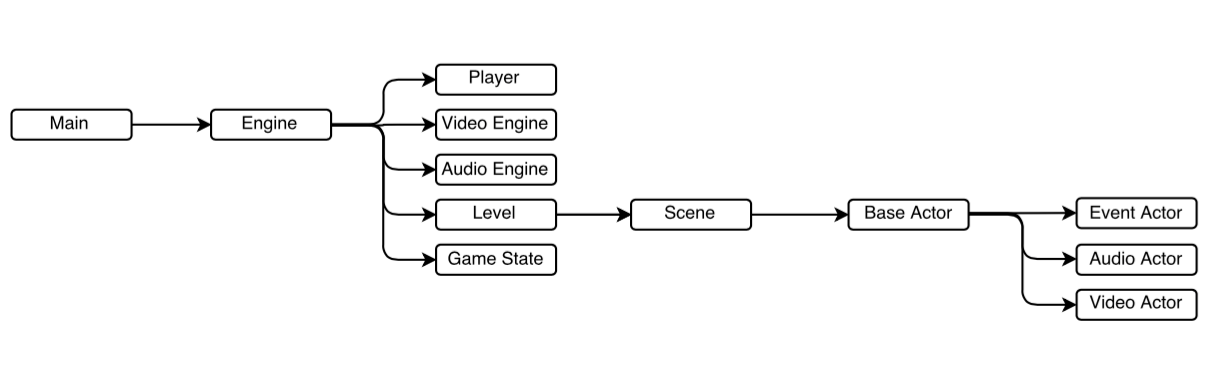
\includegraphics[scale=0.4,angle=90]{Top_down.png}
			\end{center}
	%%%
	\subsection{Dynamic Data Flow Analysis}
		\subsubsection{Flow Diagram}
			\begin{center}
				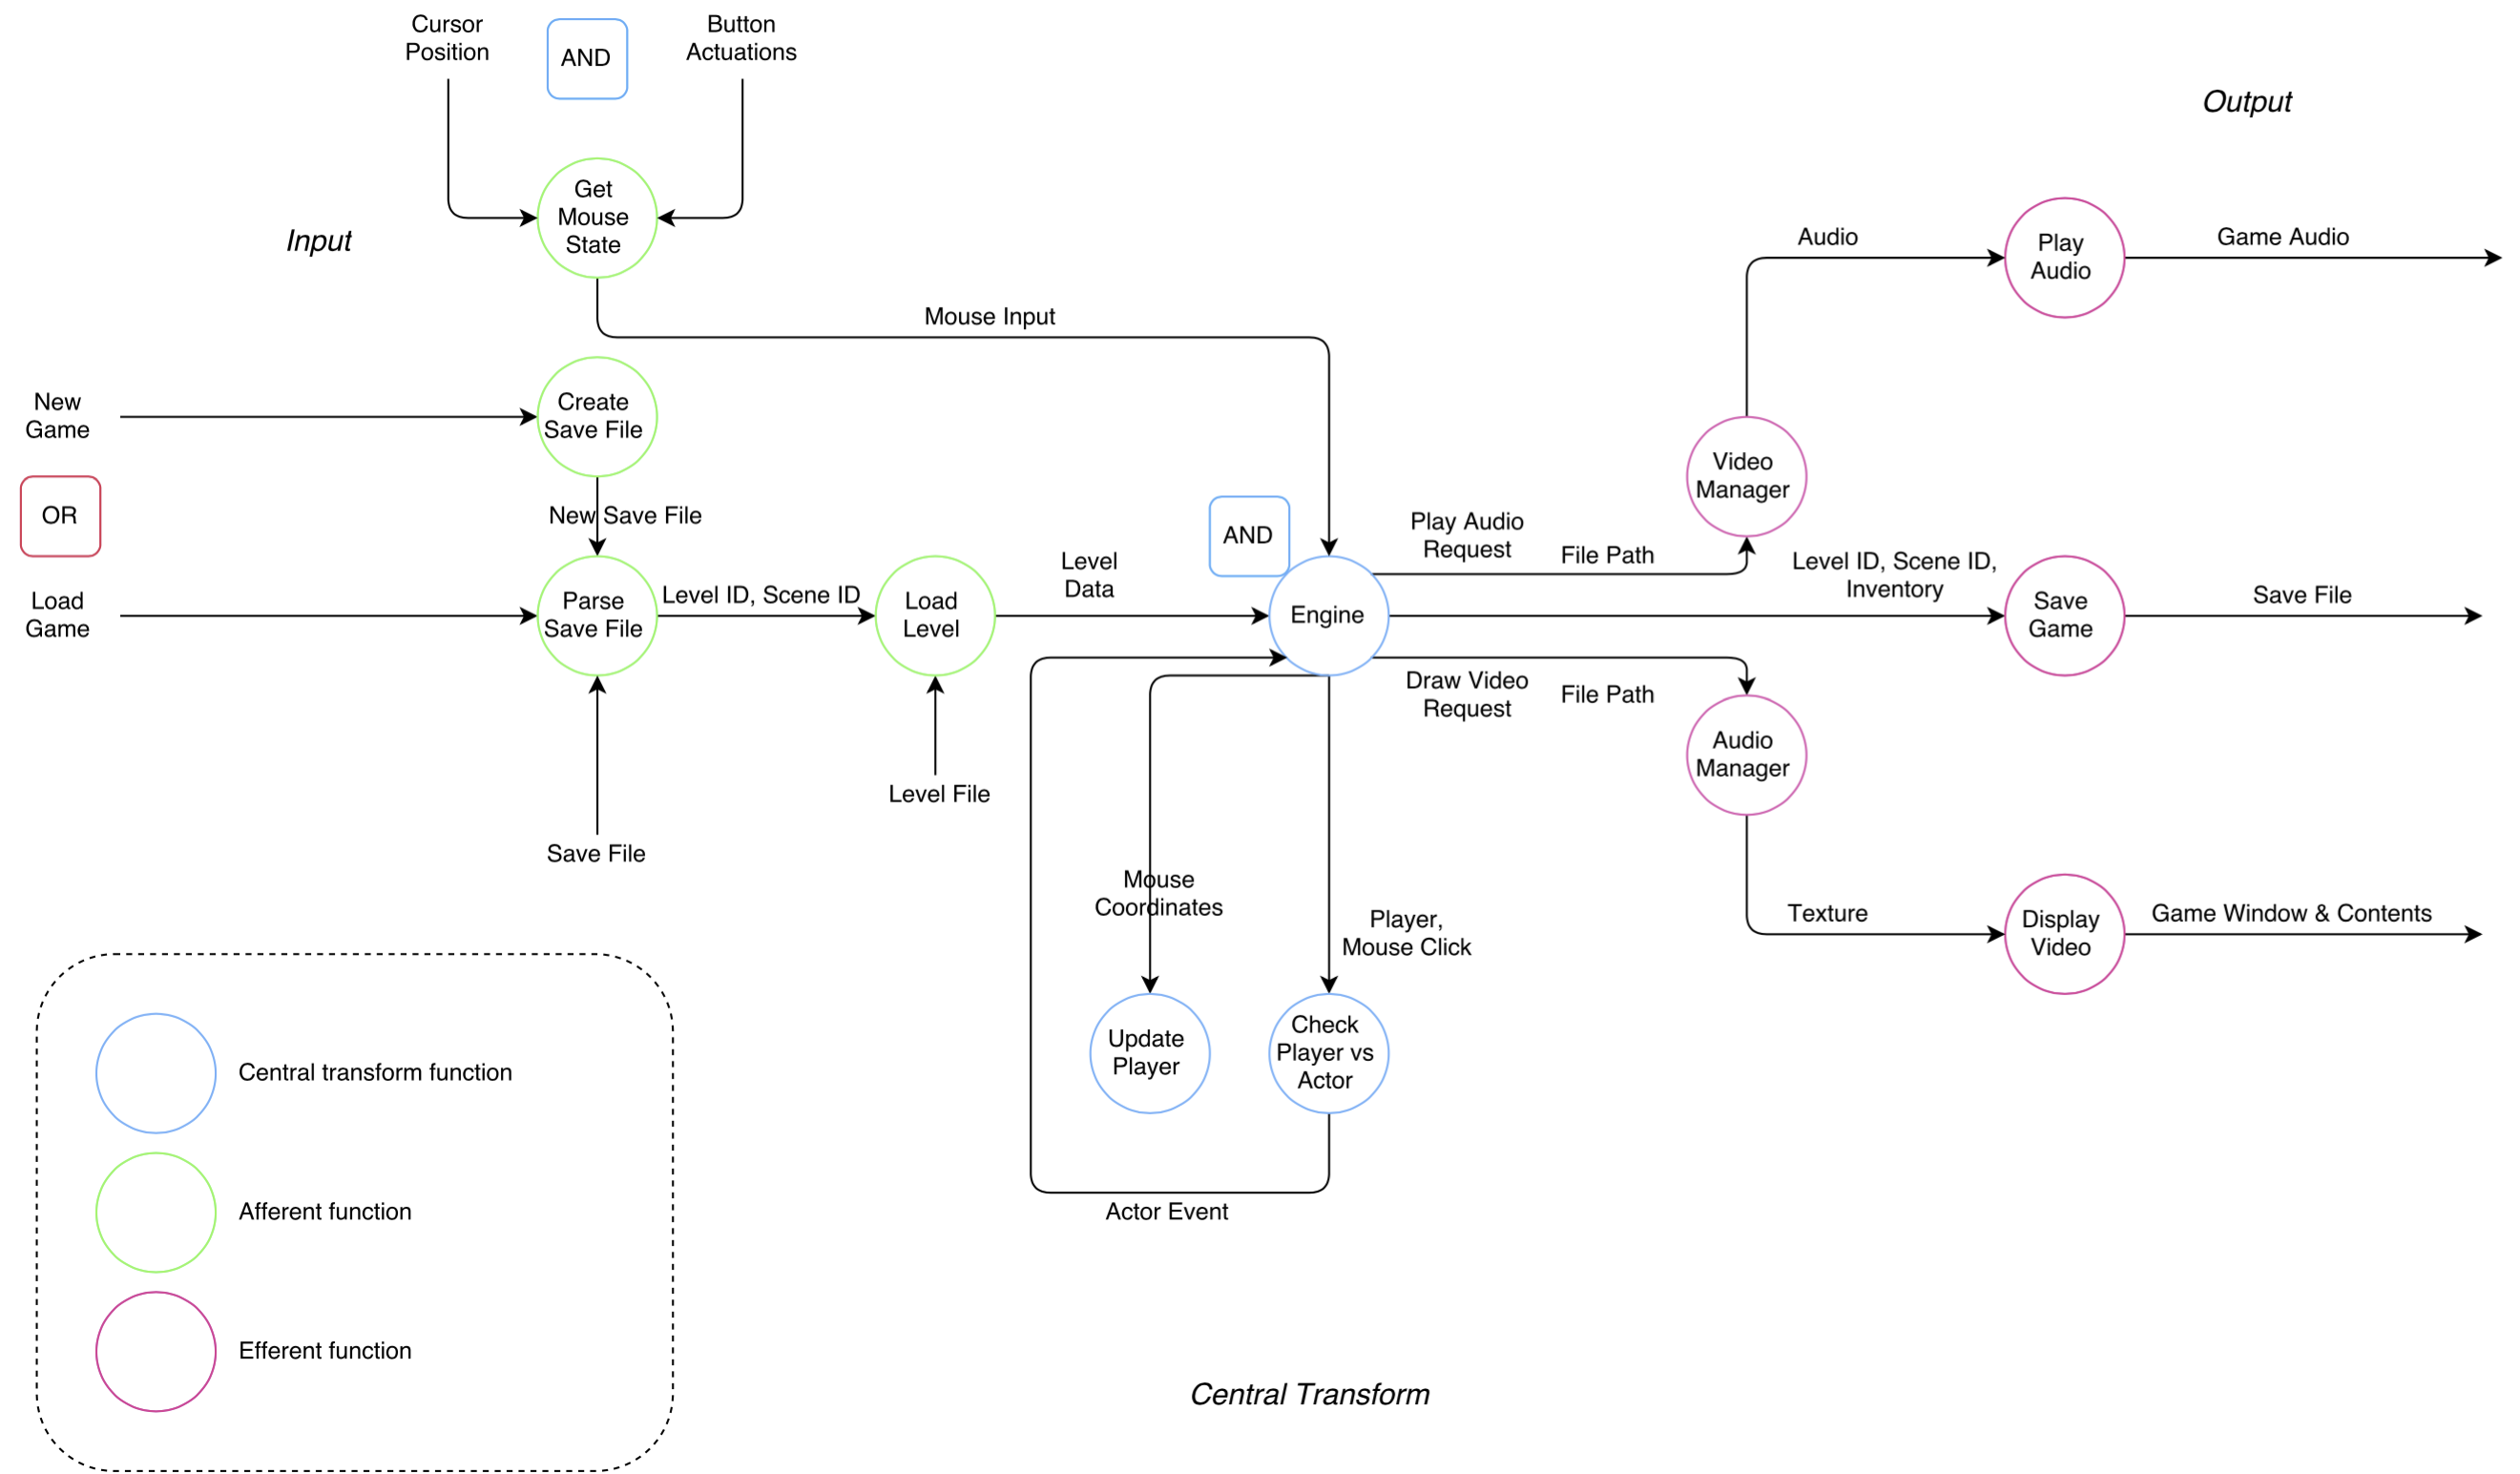
\includegraphics[scale=0.40,angle=90]{ddfFlow.png}
			\end{center}
		\subsubsection{Factored Diagram}
			\begin{center}
				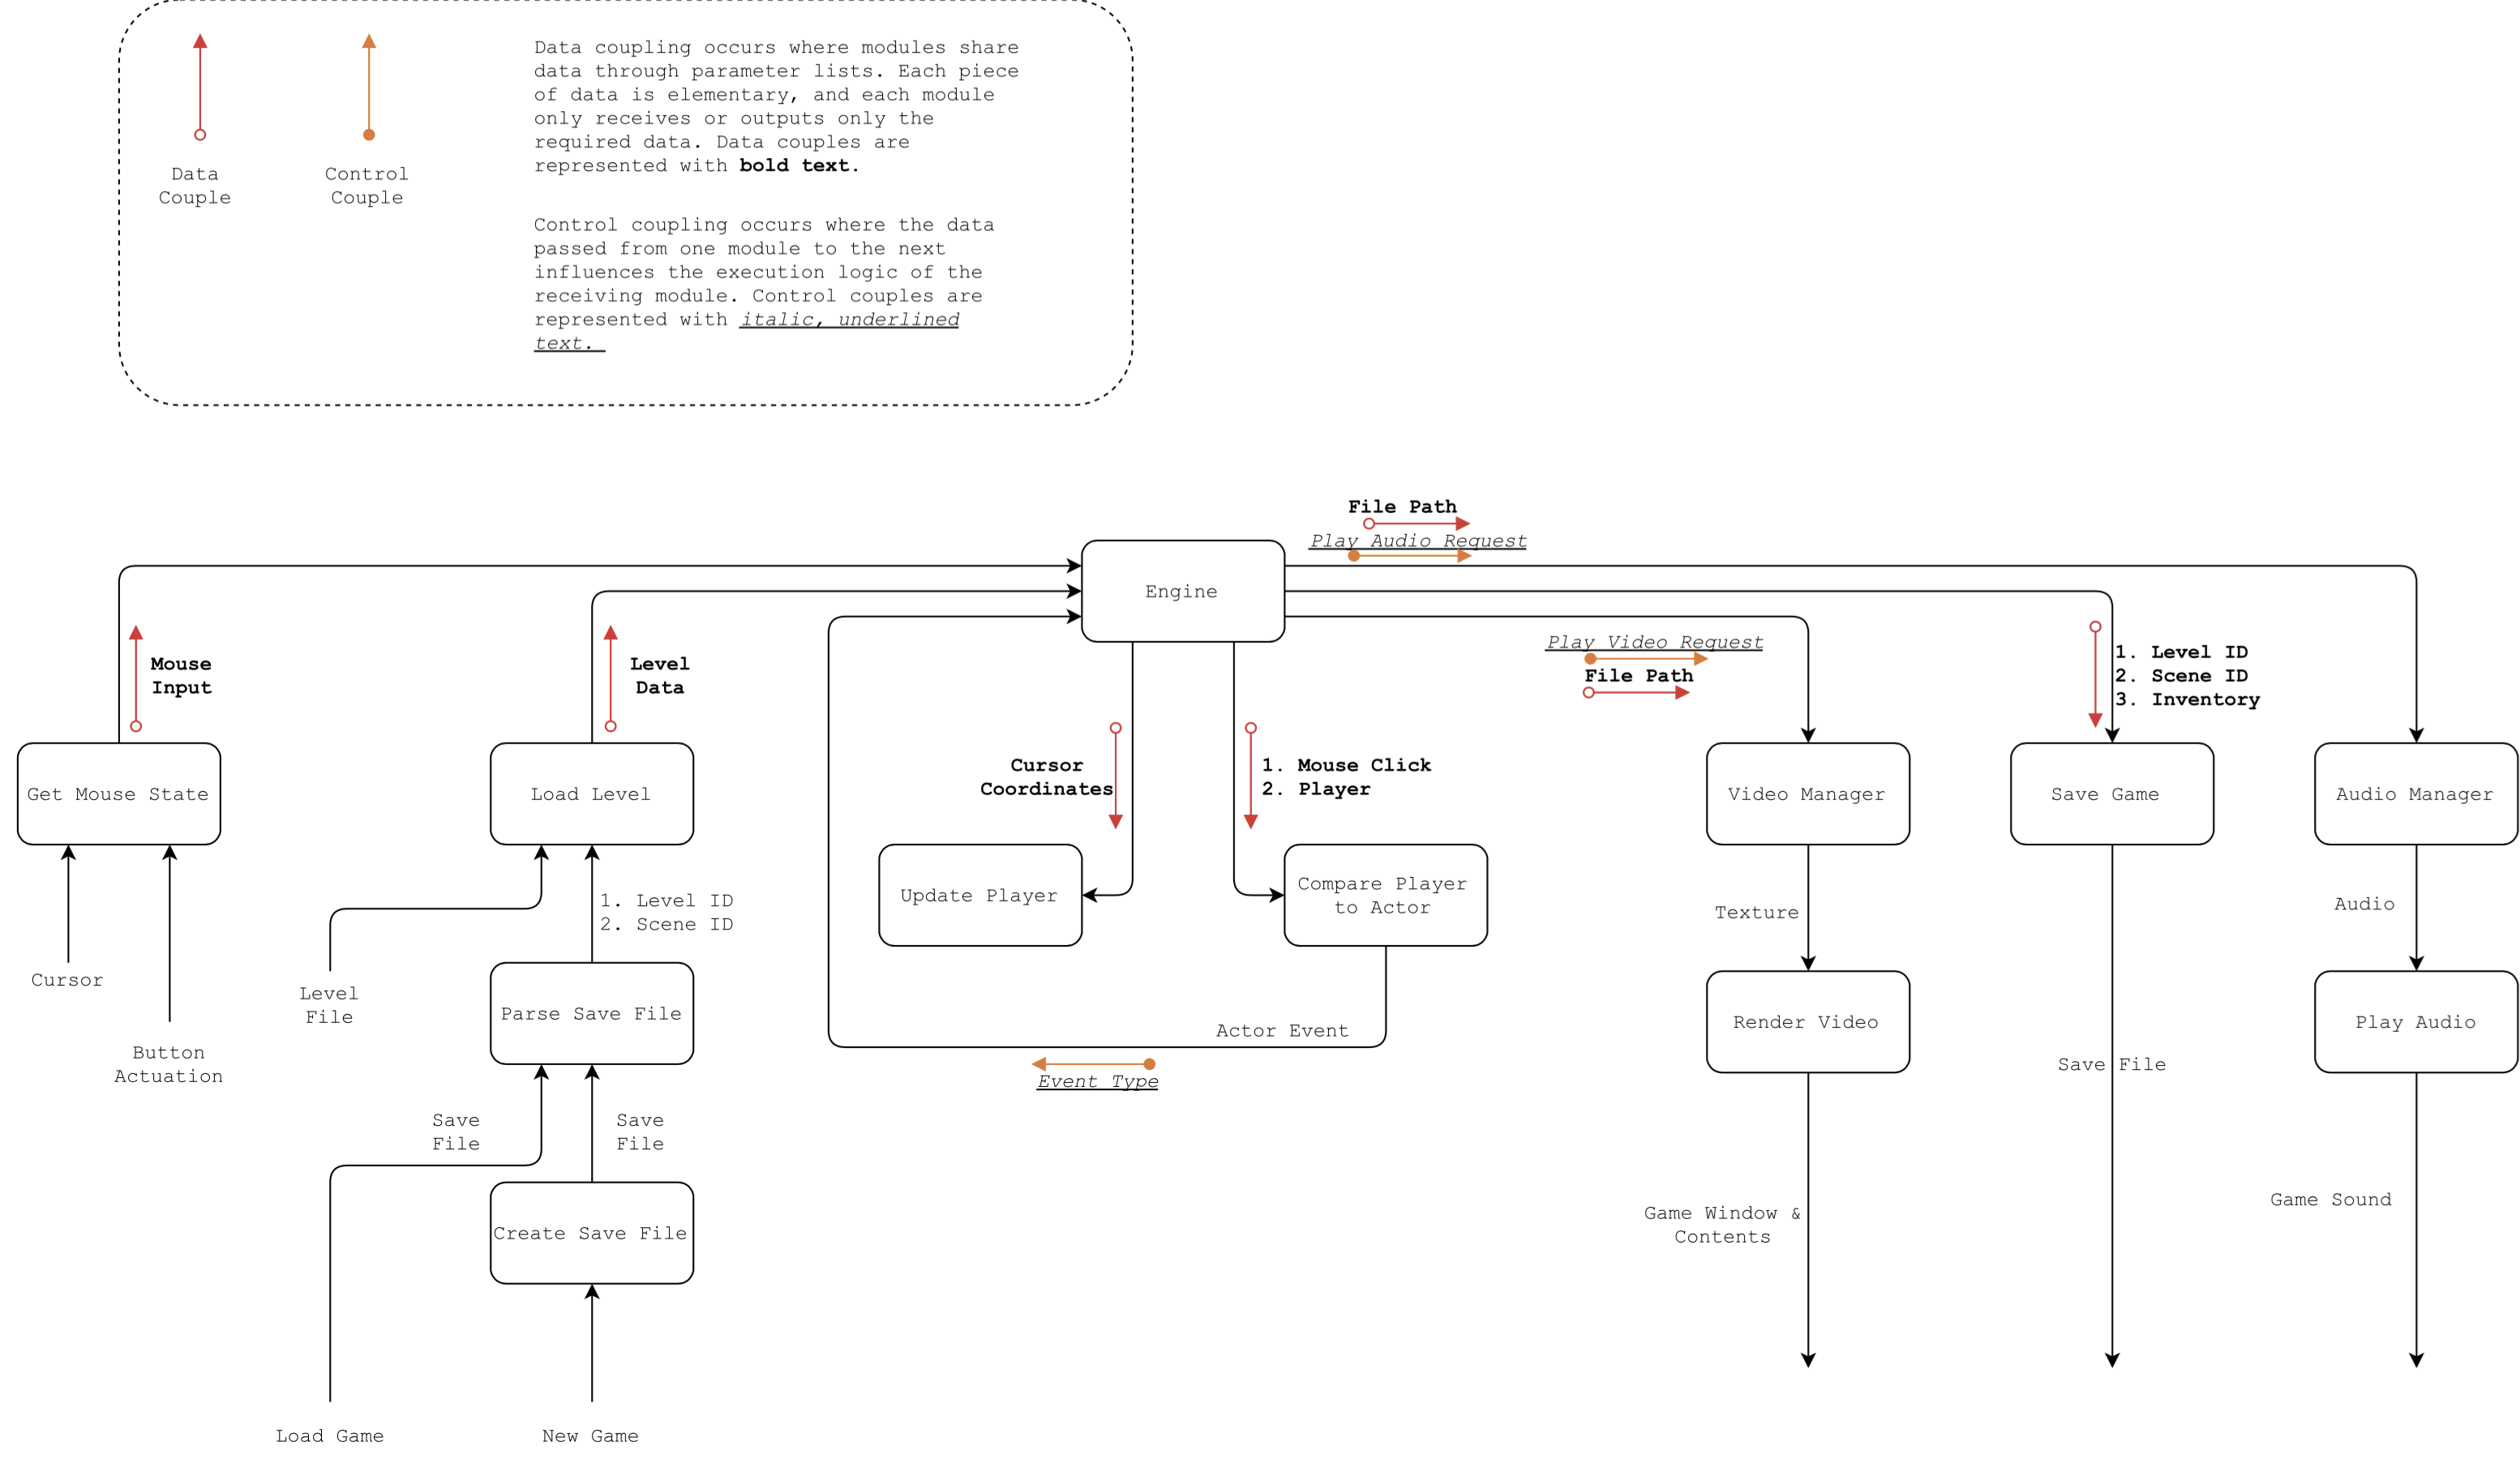
\includegraphics[scale=0.36,angle=90]{ddfFactored.png}
			\end{center}
	%%%
	\subsection{Static Data Flow Analysis}
		\subsubsection{Data Structure Diagram}
			\begin{center}
				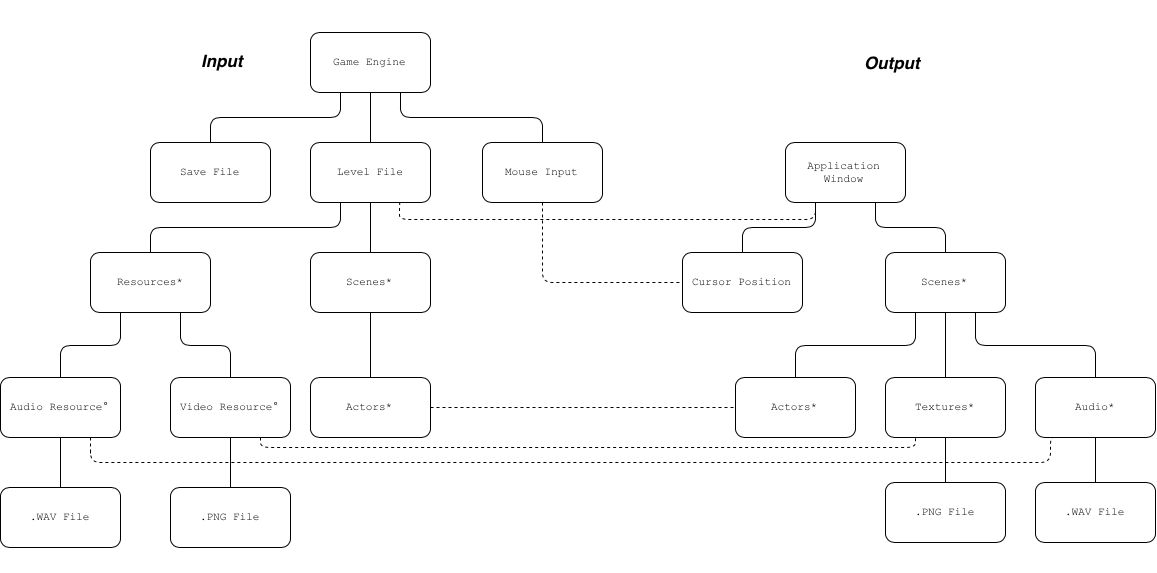
\includegraphics[scale=0.45,angle=90]{Jackson1.png}
			\end{center}
		\subsubsection{Program Structure Diagram}
			\begin{center}
				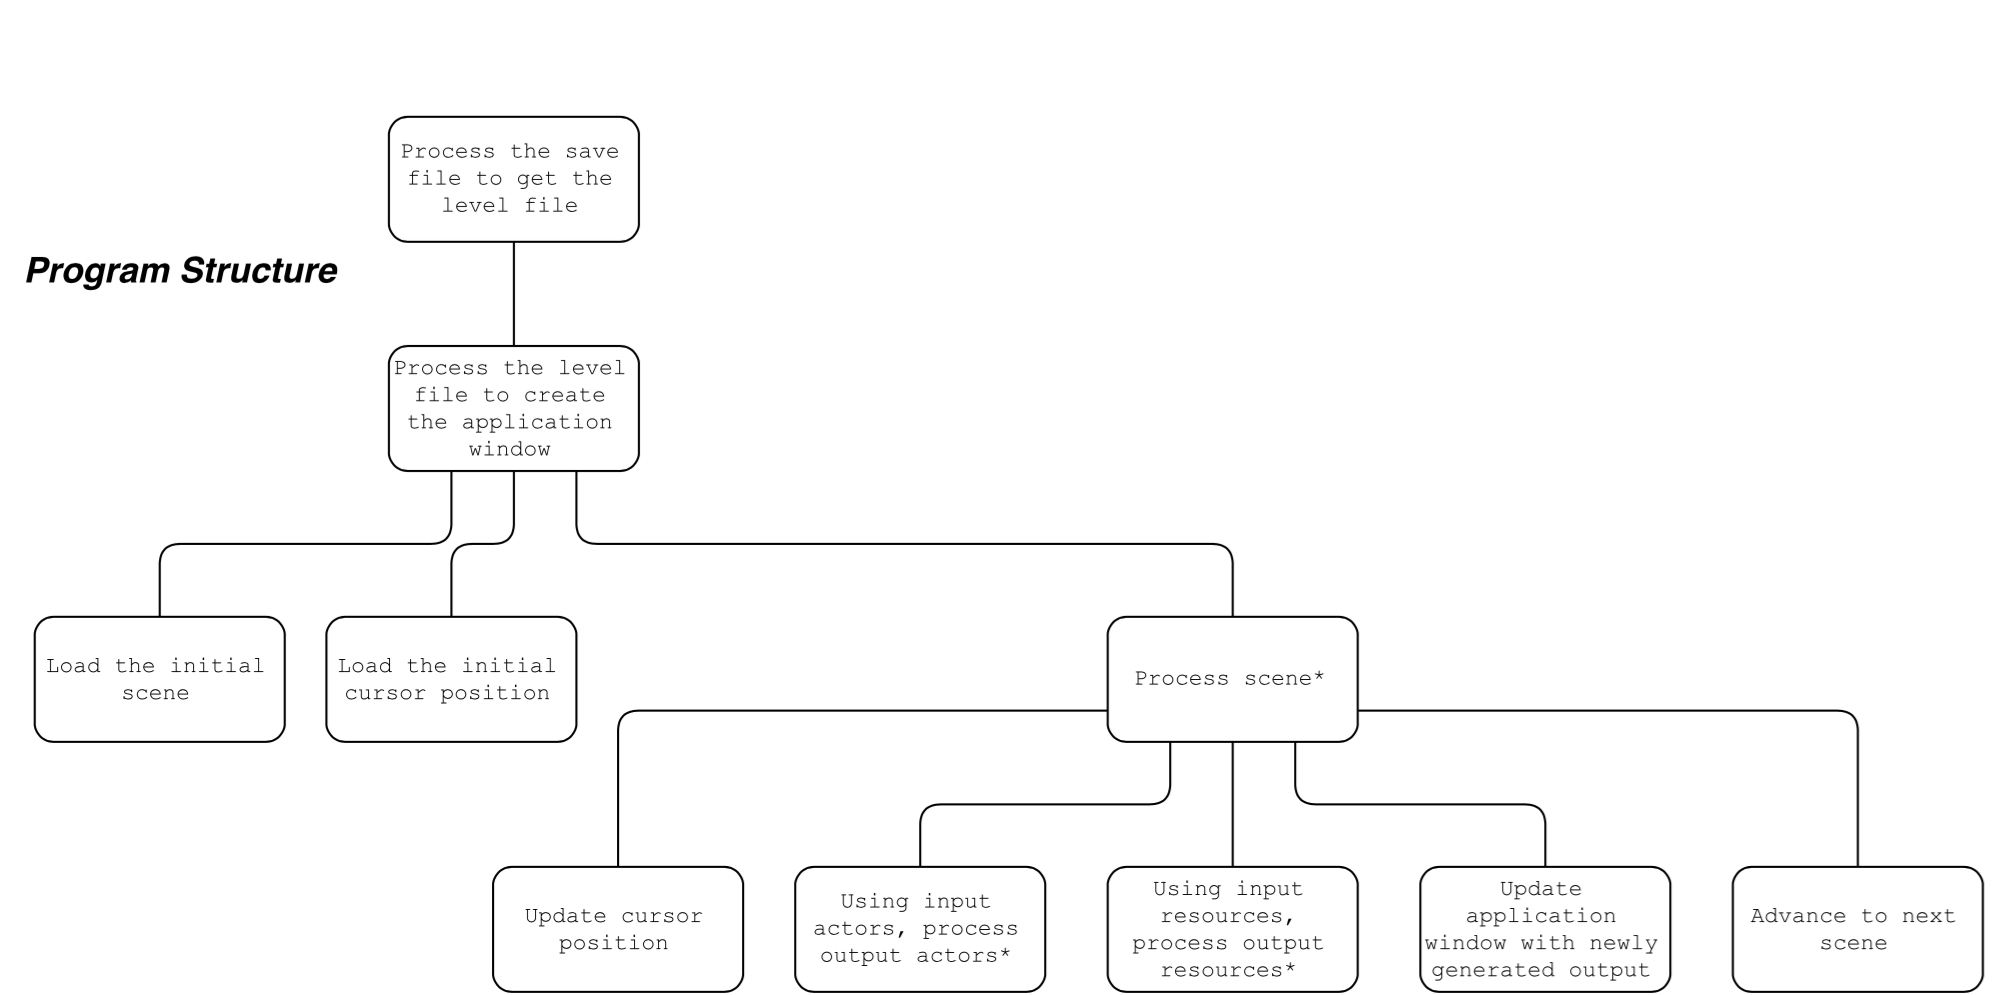
\includegraphics[scale=0.5,angle=90]{Jackson2.png}
			\end{center}
		\subsubsection{Nonprocedural Program Tasks \& Task Allocation}
			\begin{center}
				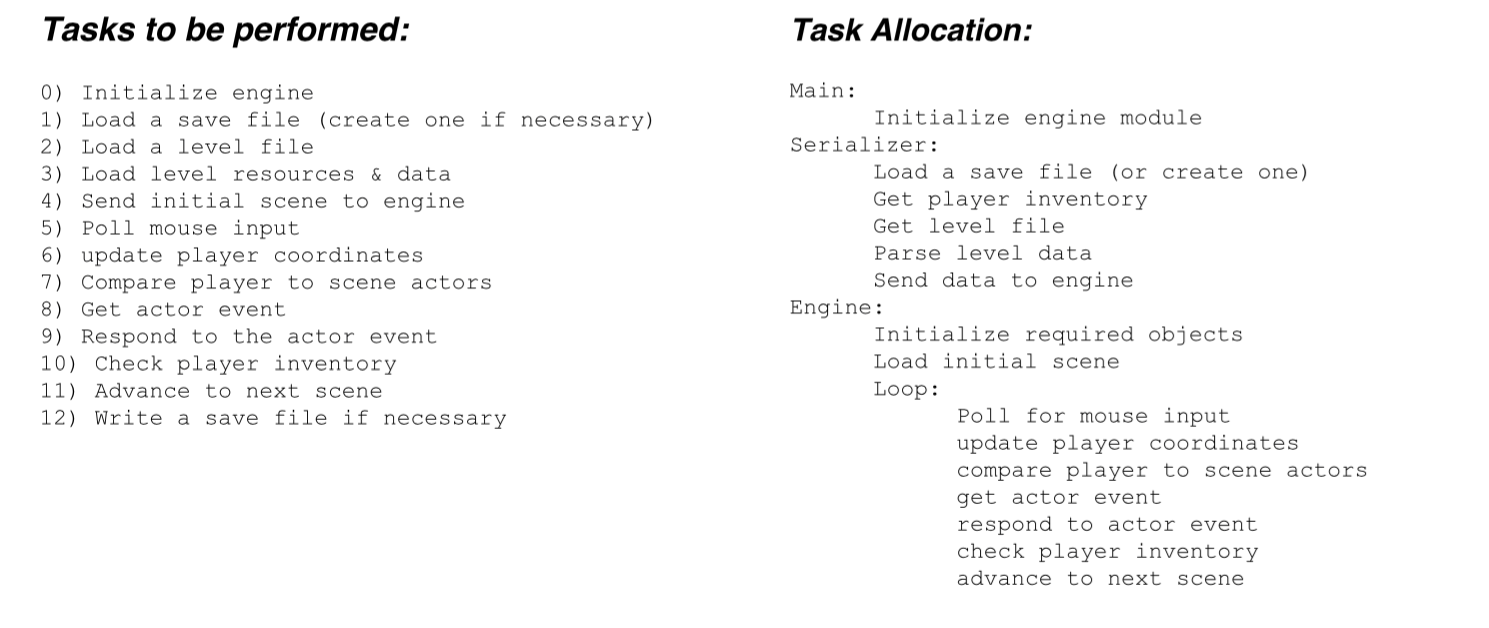
\includegraphics[scale=0.74,angle=90]{Jackson34.png}
			\end{center}
	%%%
	\subsection{Object Oriented + Unified Modeling Language}
		\subsubsection{UML Diagram}
			\begin{center}
				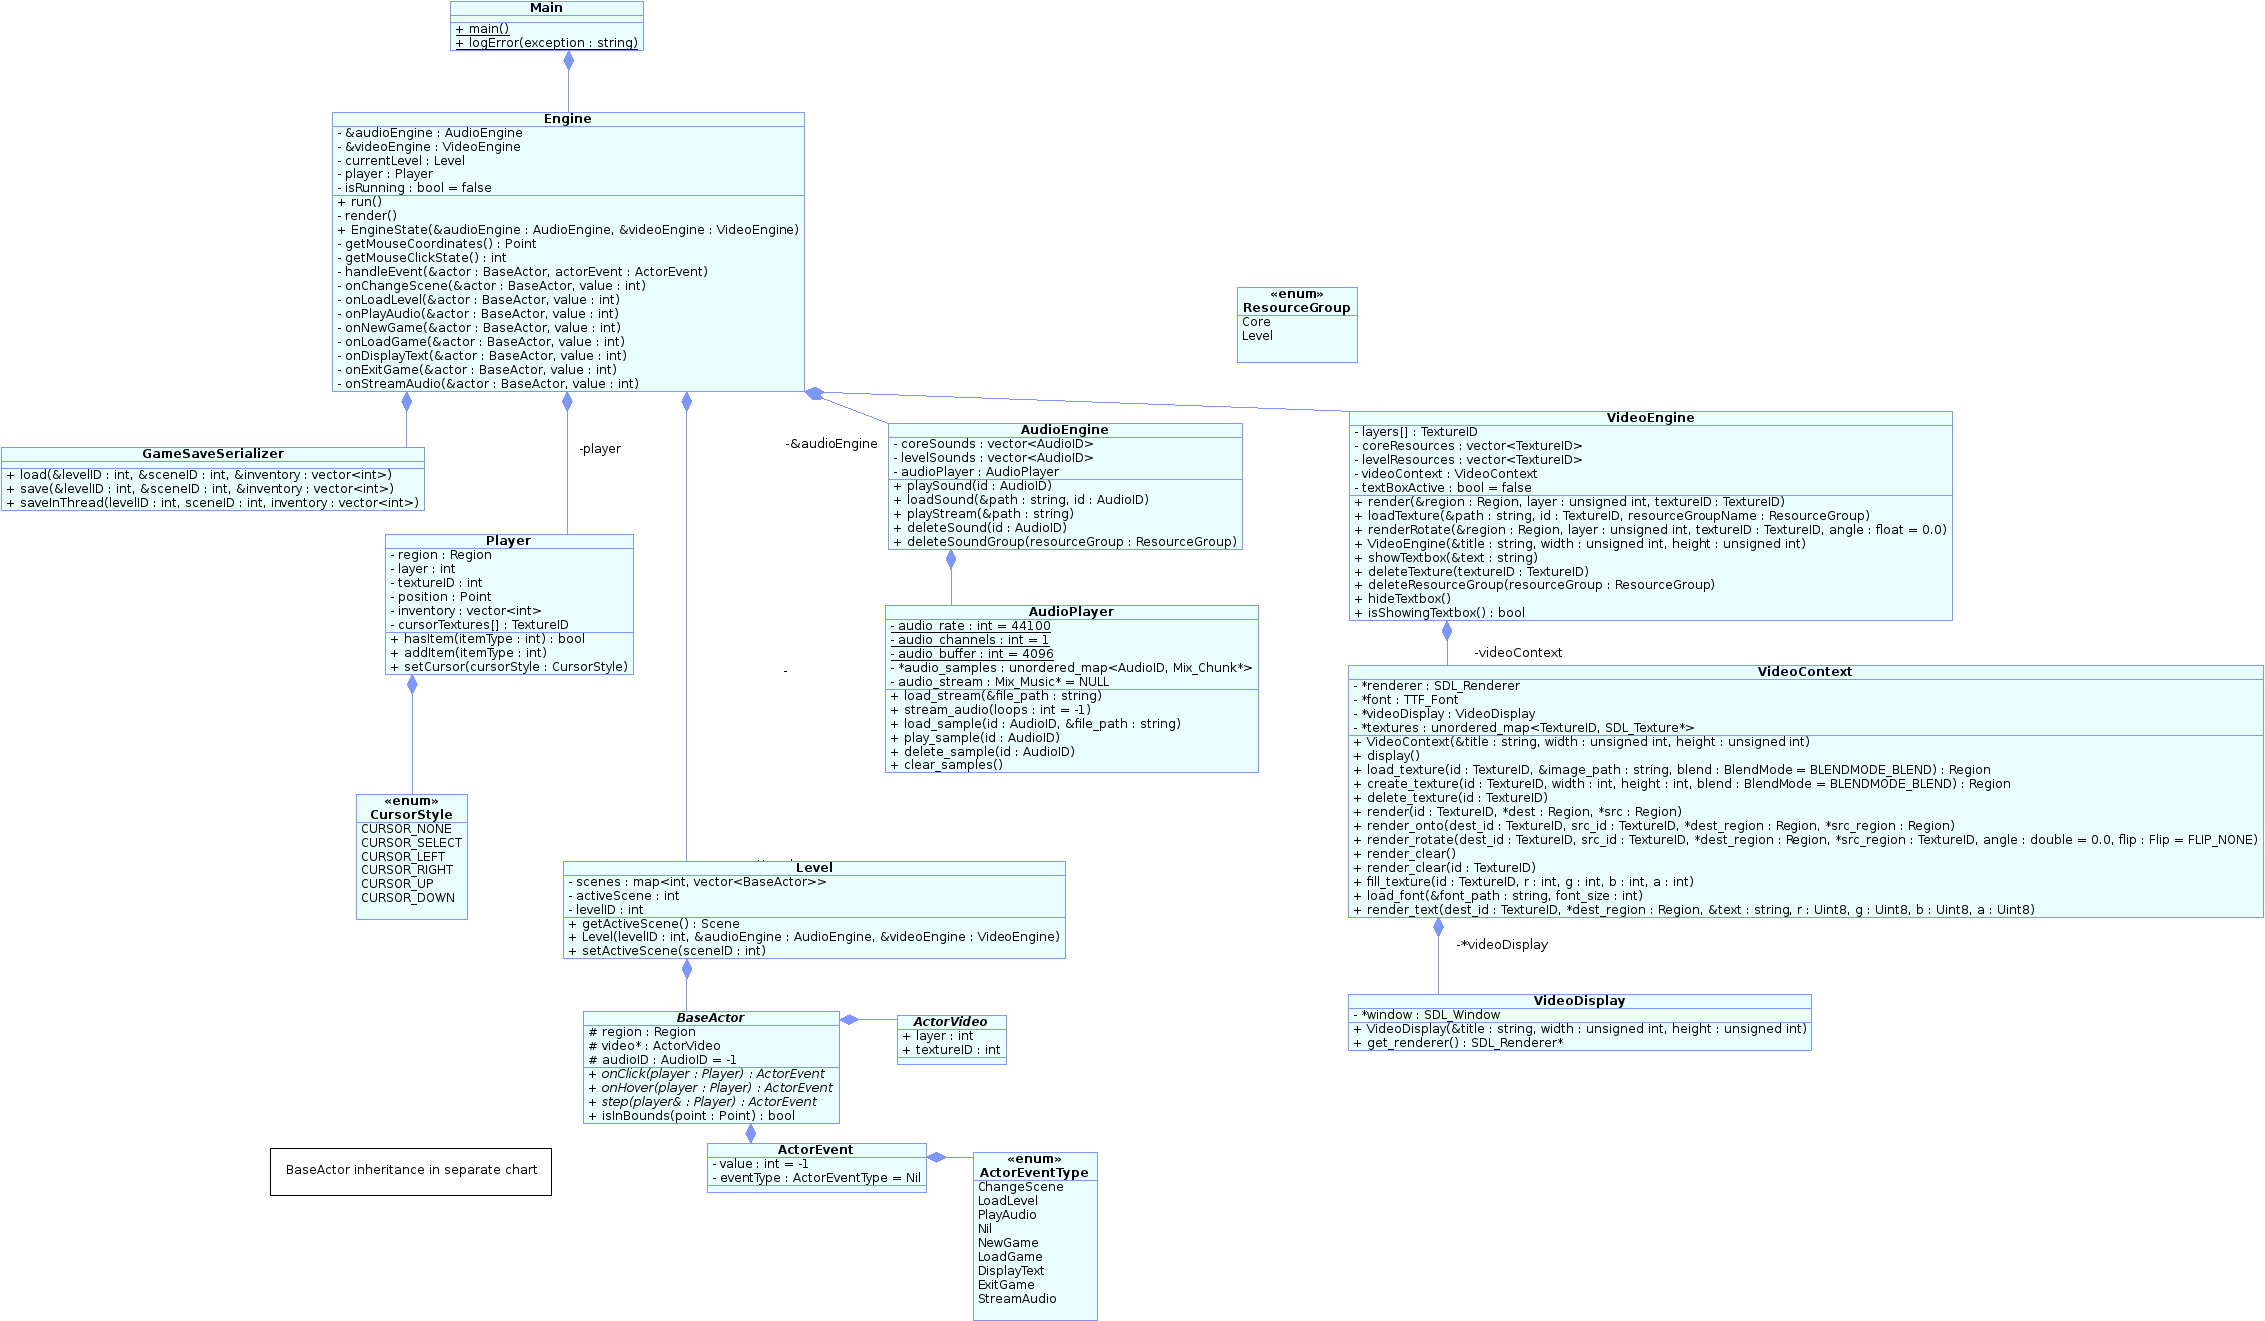
\includegraphics[scale=0.49,angle=90]{MainClasses.png}
			\end{center}
    \subsubsection{Audio / Video Sub-diagram}
      \begin{center}
				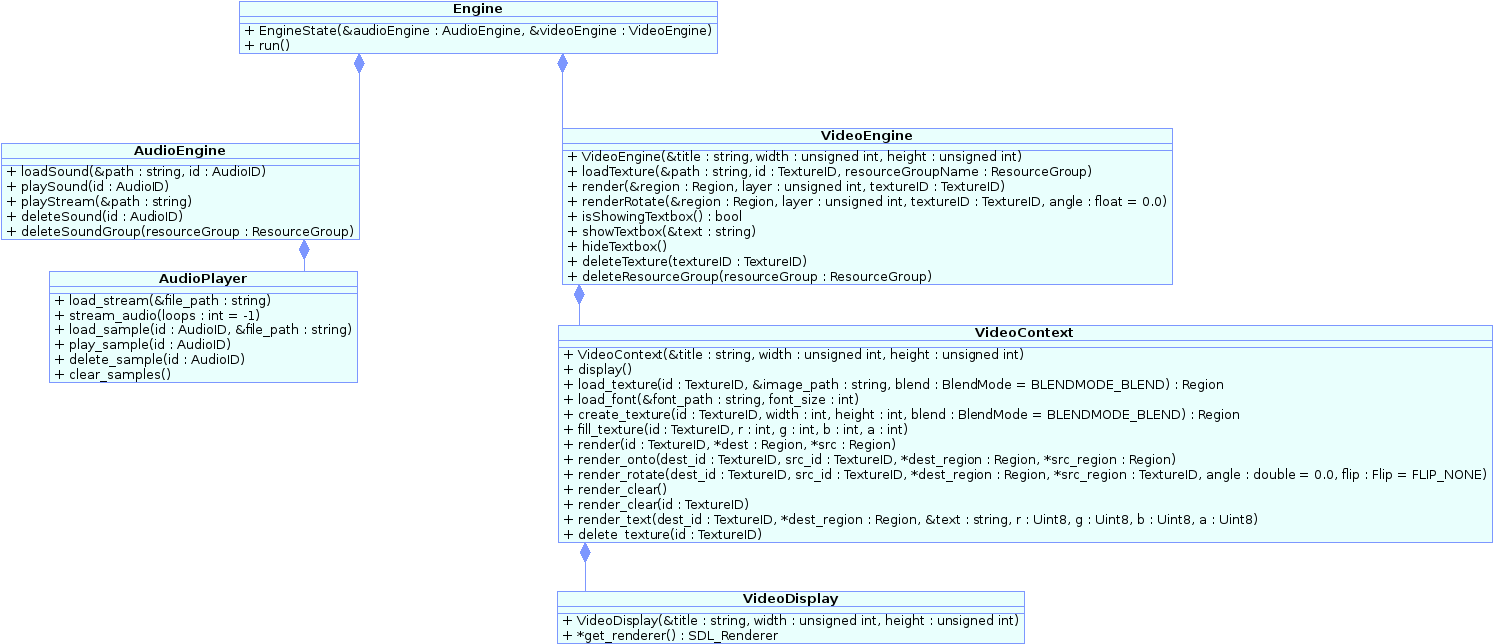
\includegraphics[scale=0.50,angle=90]{AudioVideoClasses.png}
      \end{center}
		\subsubsection{Actor Inheritance Sub-diagram}
			\begin{center}
				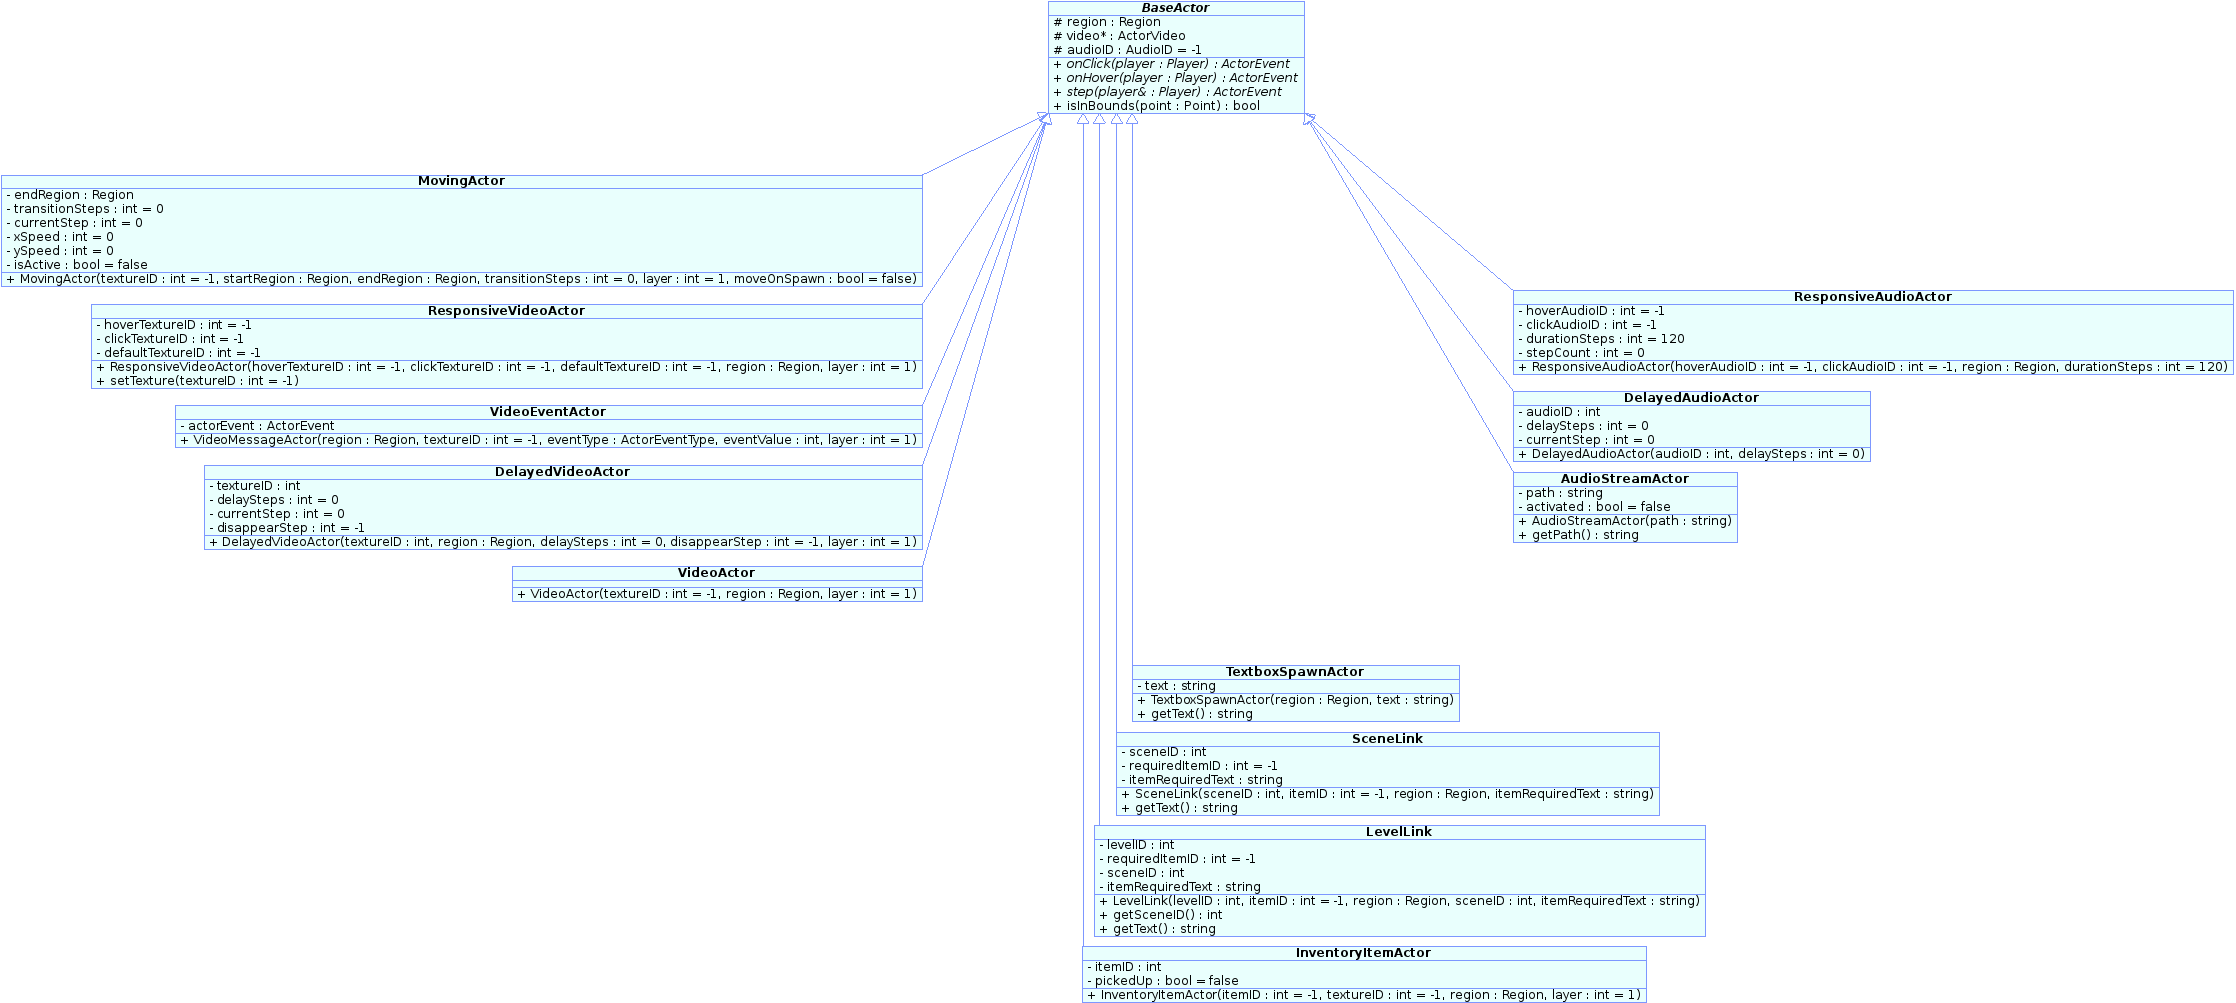
\includegraphics[scale=0.51,angle=90]{Actors.png}
			\end{center}
		\subsubsection{Timing Diagrams}
			\paragraph{Handle Actor Event}
				\begin{center}
					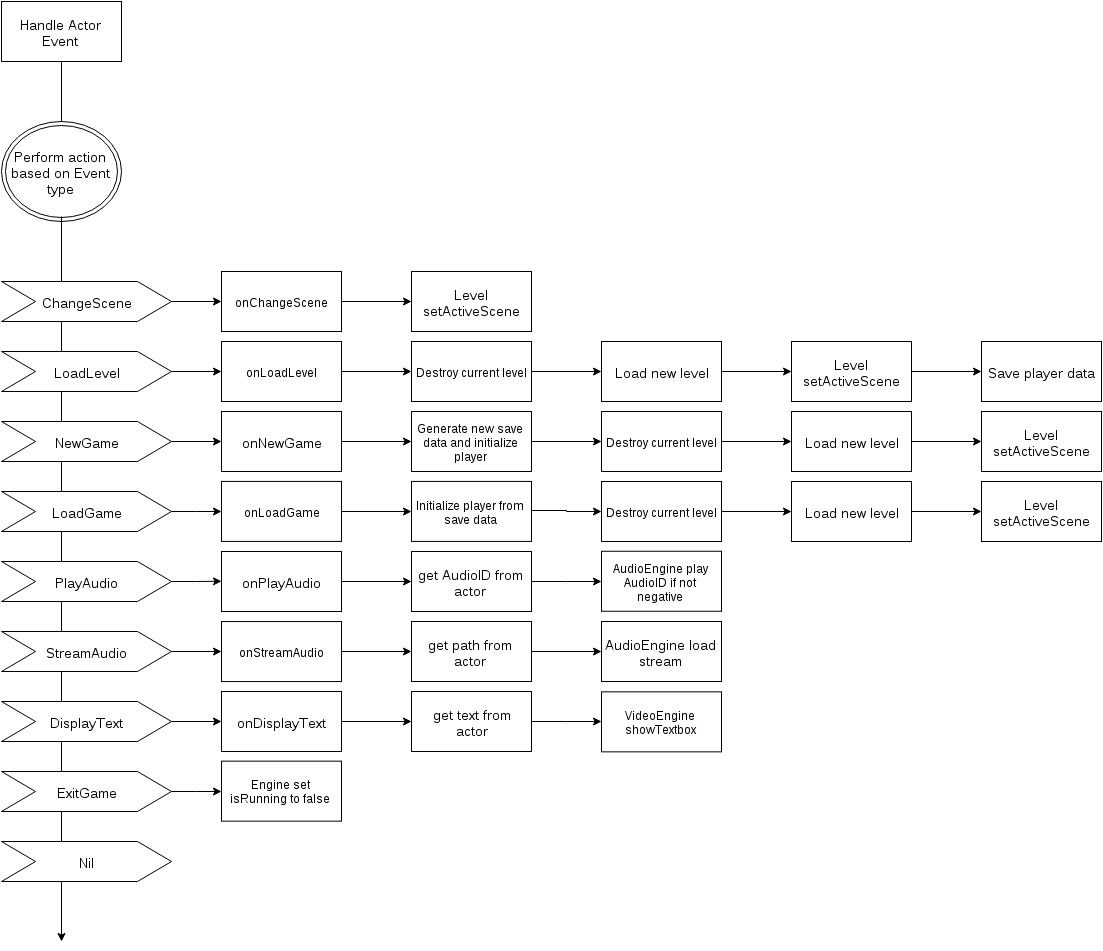
\includegraphics[scale=0.48,angle=90]{handle-actor-event.png}
				\end{center}
			\paragraph{Load Level}
				\begin{center}
					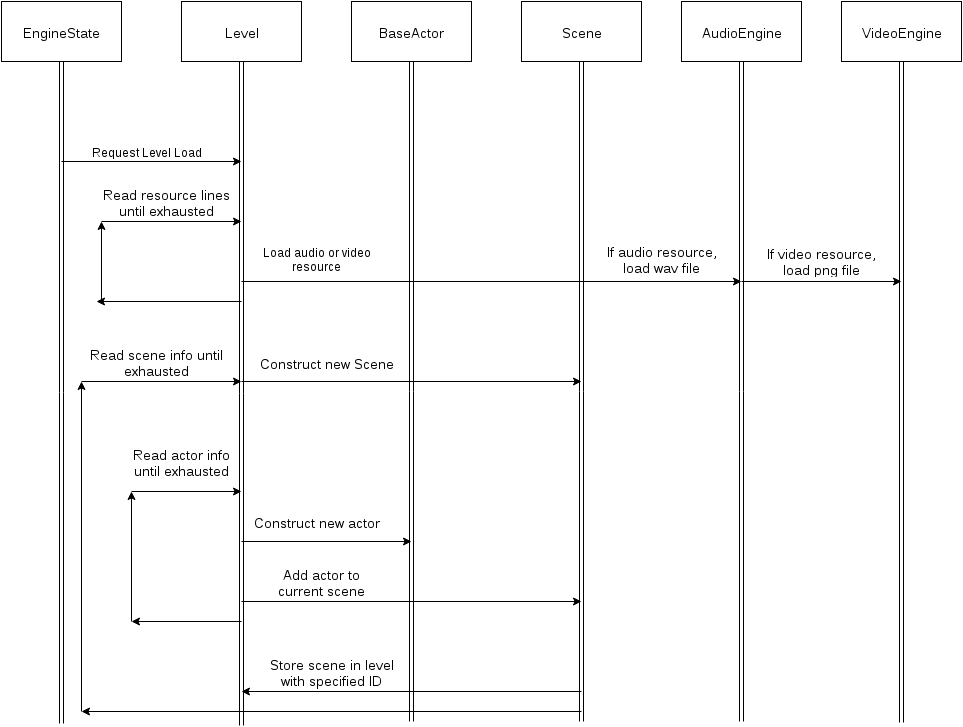
\includegraphics[scale=0.58,angle=90]{load-level.png}
				\end{center}
			\paragraph{Main Loop}
				\begin{center}
					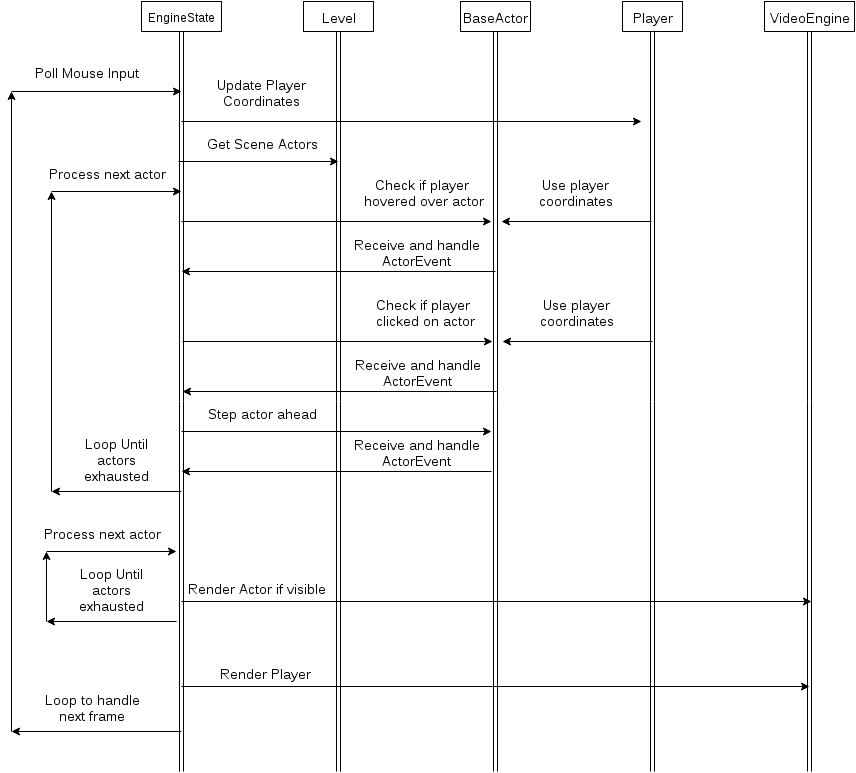
\includegraphics[scale=0.54,angle=90]{main-loop.png}
				\end{center}
%
% Appendix B - Story & Level Progression
%
\newpage
\section{Appendix B: Level Progression \& Miscellany}
	\subsection{Level Progression Diagram}
		\begin{center}
			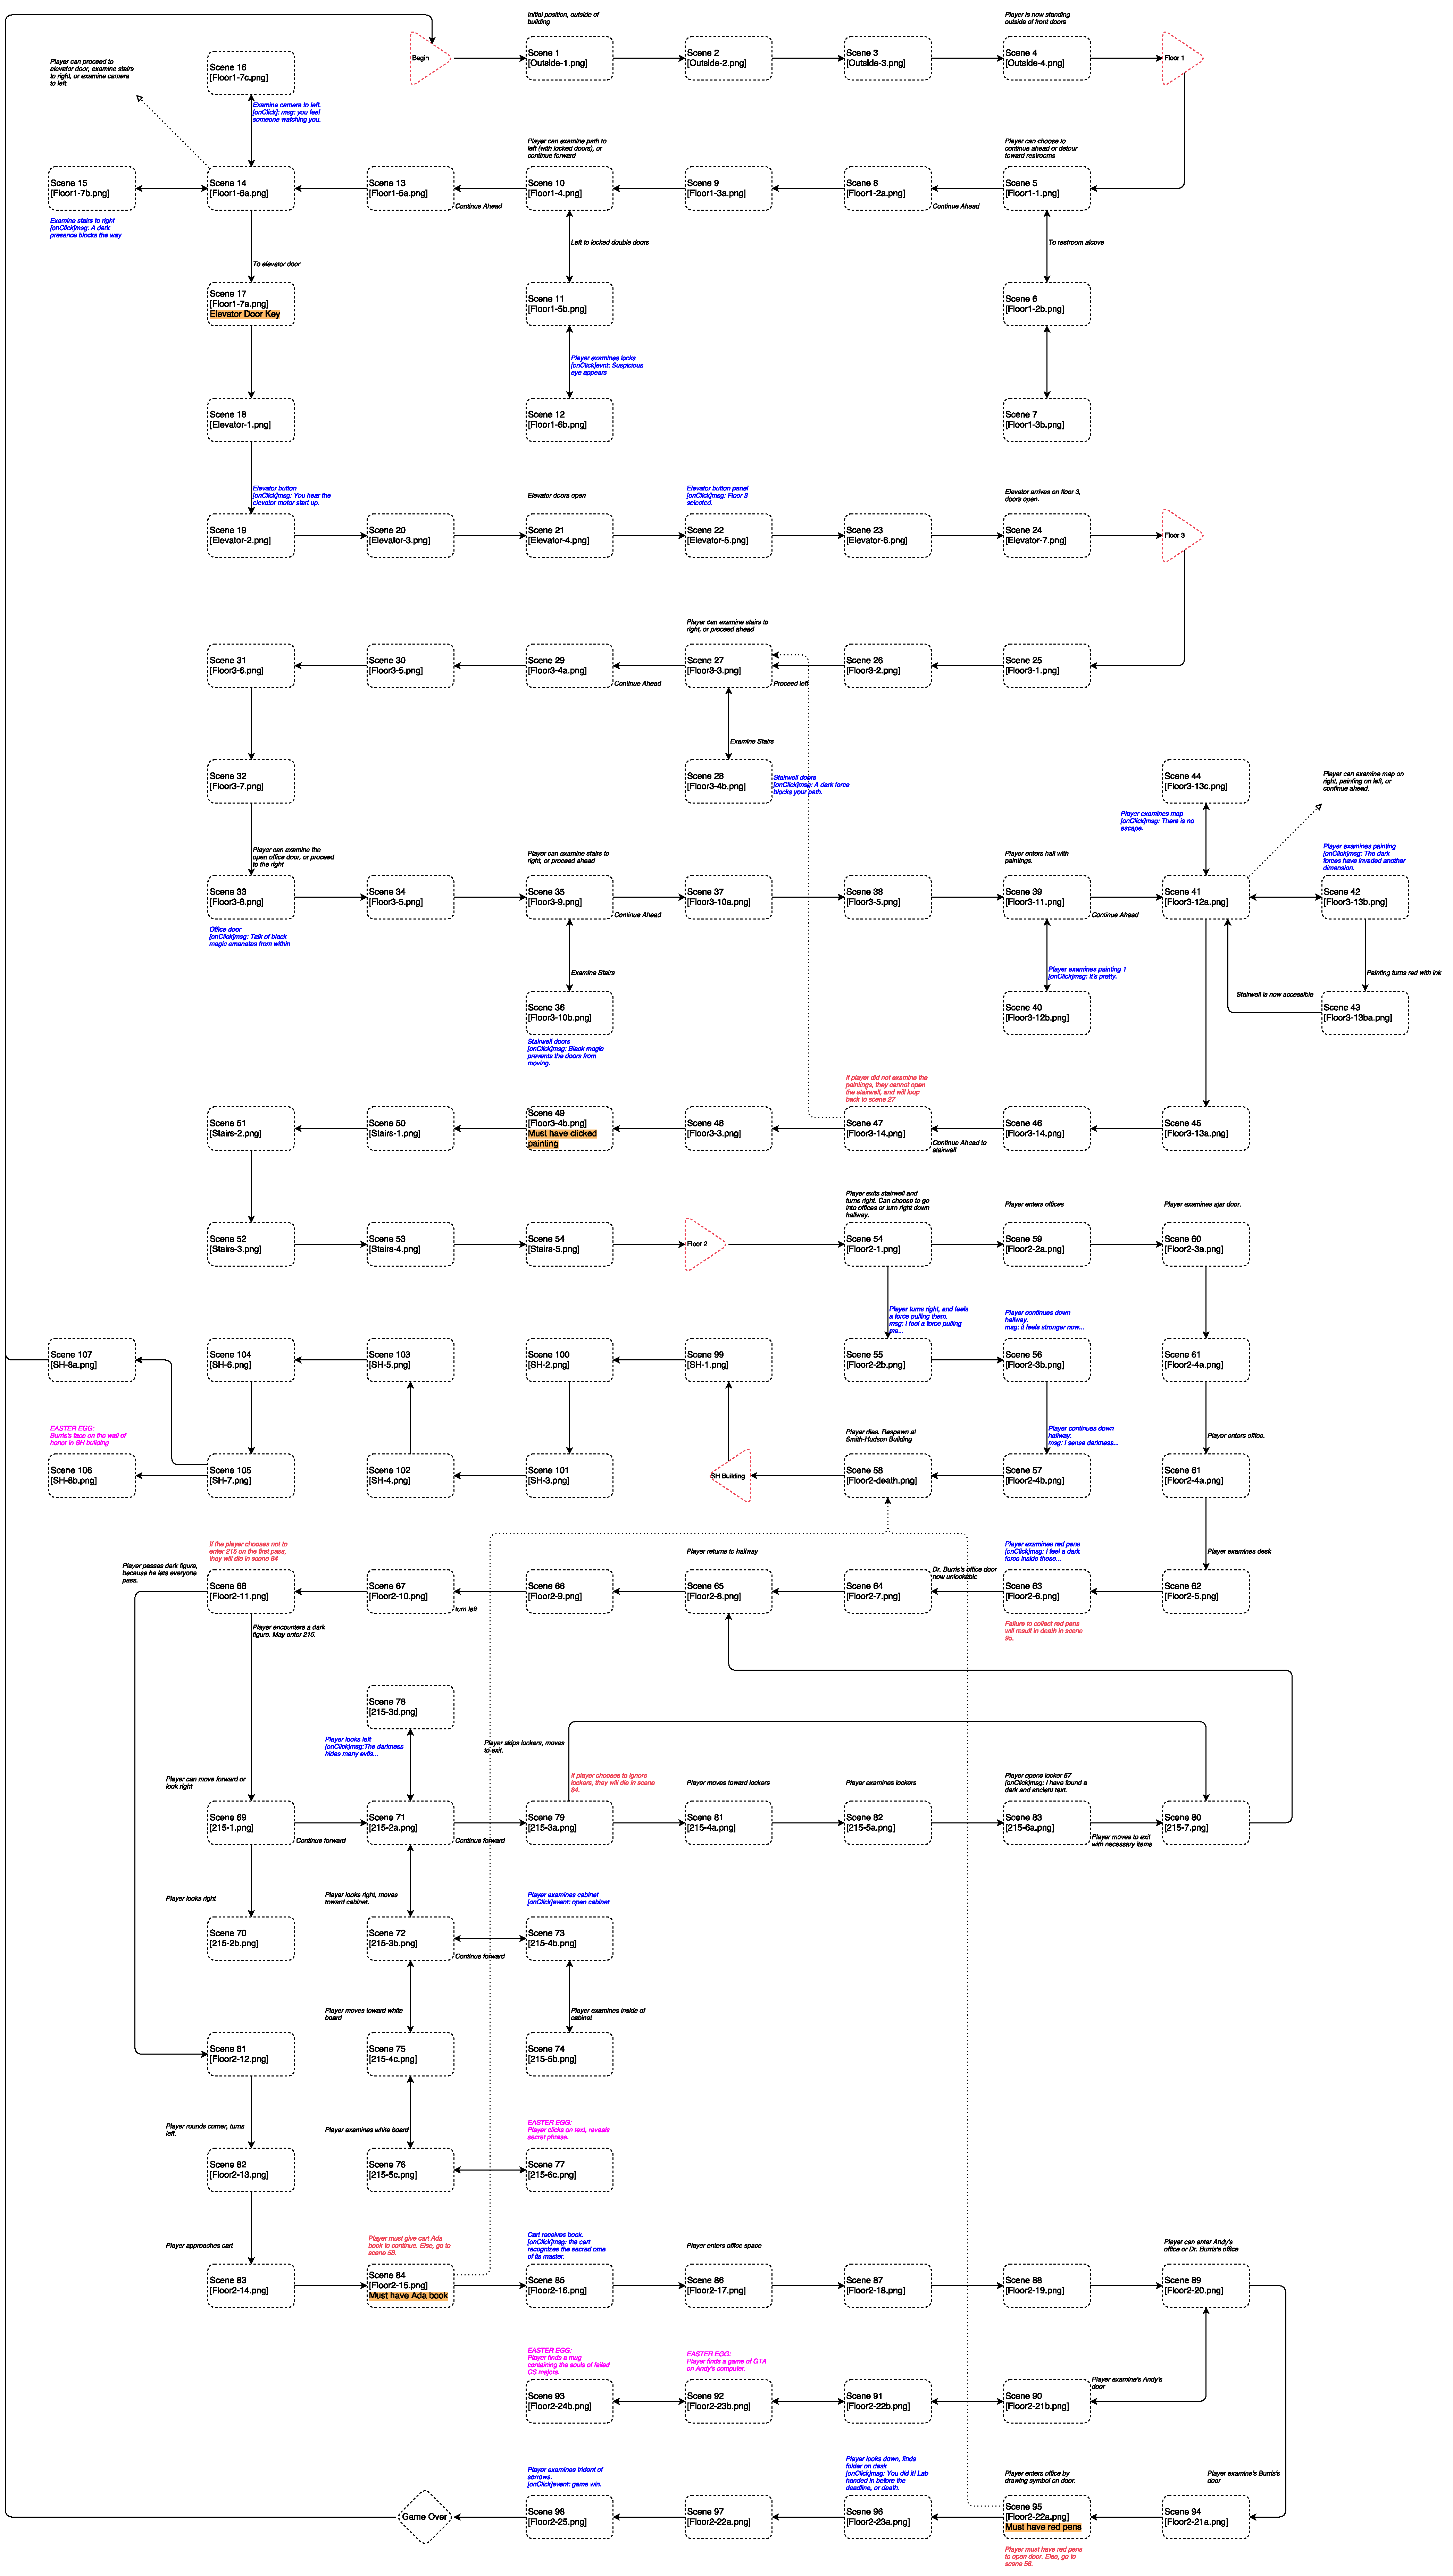
\includegraphics[scale=0.15]{LevelProgression.pdf}
		\end{center}
		A full sized level progression diagram has been attached separately. It is included here merely for completeness, though it can be magnified and viewed using a suitable PDF viewer on a computer. 
	\subsection{Miscellany} 

%%%%%%%%	
\end{document}
